\chapter{Inleiding tot Grafentheorie}

Grafen kunnen dikwijls gebruikt worden als abstractie om een concreet
probleem op te lossen en zijn dan ook een context waarbinnen veel
algoritmen zijn ontwikkeld: een kortste-pad zoeken (gps), een
opspannende boom (optimalisatie van netwerken), grafenkleuring
(registerallocatie door een compiler), systematisch doorlopen van een
boom (een zoekboom of een spelboom), maximale netwerkflow, kringen
allerhande ... Het is daarom goed om de abstracte context van grafen
wat formeler te bestuderen. Dit hoofdstuk behandelt o.a.
\begin{inparaenum}[~~]
\item 
definities i.v.m. grafen en voorbeelden van speciale grafen;
\item 
vlakke grafen - formule van Euler, $K_3$ en $K_{2,2}$ als minimale niet-vlakke
grafen;
\item
kringen (Euler en Hamilton);
\item 
gewogen grafen;
\item
minimaal opspannende (Steiner) boom (Kruskal en Prim);
\item
het maximale flow en het SCCS algoritme;
\item
grafen kleuren;
\item
problemen modelleren met grafen.
\end{inparaenum}




\section{Inleiding}

Informeel is een graaf een tekening van punten (die we knopen noemen)
die verbonden kunnen zijn door lijnen (bogen). Later defini\"eren we
alles meer formeel.

\subsection{De drie munten}

Drie munten liggen op tafel, alle met kop (K) omhoog. Je mag
verschillende keren de volgende handeling uitvoeren: neem twee munten,
draai ze om en leg ze terug. Gevraagd wordt: is het mogelijk dat na
een aantal van zulke handelingen alle munten met de muntkant (M) boven
liggen?

E\'{e}n van de manieren om dit (type van) probleem op te lossen, is een
graaf te tekenen met de mogelijke configuraties van de 3 munten als
knopen; tussen twee configuraties wordt enkel een verbinding getekend
als het mogelijk is om van de ene configuratie naar de andere te gaan
door de spelregels te volgen: twee munten tegelijk omkeren. We bekomen de
graaf in Figuur~\ref{munten}.

\begin{figure}[ht]
\begin{center}
\includegraphics[width=0.5\linewidth,keepaspectratio]{munten}
\end{center}
\caption{De graaf met de 3 munten \label{munten}}
\end{figure}

Uit de graaf is vlug duidelijk dat het niet mogelijk is om van de KKK
configuratie tot MMM te komen terwijl de spelregels gerespecteerd
worden, omdat je niet van KKK naar MMM kan gaan door verbindingen te
volgen. KKK en MMM liggen in een verschillende component van de graaf.


\subsection{De wolf, de geit en de kool.}

Een boer bezit een wolf, een geit en een kool; hij leeft aan de
linkeroever van een rivier en wil al zijn bezittingen naar de overkant
brengen. Hij heeft een bootje, maar dat is niet groot genoeg om meer
dan \'{e}\'{e}n van zijn bezittingen tegelijk naar de overkant te
varen. Hij zou natuurlijk drie keer over kunnen varen met telkens
\'{e}\'{e}n van zijn bezittingen, maar zogauw hij de geit en de kool
alleen laat, eet de geit de kool op; en hetzelfde geldt voor de wolf
en de geit: dat wil de boer natuurlijk vermijden. Bestaat er een
manier om alles naar de overkant te brengen?

Om dit op te lossen, kan je natuurlijk alle mogelijkheden
proberen en dan zit je met het probleem van boekhouding. Hier is een
systematische manier om het te doen: schrijf eerst alle mogelijke
situaties neer; vermits een situatie volledig vastligt als je weet wat
op welke oever is, kan je dat doen door de voorstelling BGK te
gebruiken voor de situatie: de boer, de geit en de kool zijn op de
linkeroever. Sommige situaties zijn a priori verboden: GK zou willen
zeggen dat de geit en de kool op de linkeroever zitten (en de boer en
de wolf op de rechteroever of onderweg in het bootje) en dat is
verboden, want de geit zou de kool opeten. Alle situaties zijn dus
neer te schrijven als in Figuur~\ref{BWGK1}, waarbij $\ast$
gebruikt wordt om aan te duiden dat niets zich op de linkeroever
bevindt.

\begin{figure}[ht]
\mbox{
\hspace{1cm}
\subfigure[De mogelijke situaties voor de boer, de wolf, de geit en de kool ]{\includegraphics[height=0.12\textheight,keepaspectratio]{BWGK1} \label{BWGK1}}\hspace{2.5cm}
\subfigure[De graaf voor de wolf, de geit en de kool ]{\includegraphics[height=0.12\textheight,keepaspectratio]{BWGK2} \label{BWGK2} }
}
\caption{De boer, de wolf, de geit en de kool}
\end{figure}

Vervolgens verbinden we elke twee situaties $\alpha$ en $\beta$ als de
boer door overvaren - en eventueel \'{e}\'{e}n van zijn bezittingen
mee te nemen - de situatie $\alpha$ in $\beta$ kan wijzigen. We
verkrijgen dan de graaf in Figuur~\ref{BWGK2}.  Het probleem is nu
herleid tot de vraag: bestaat er een pad langs de lijnen van de graaf
in Figuur~\ref{BWGK2} van punt BWGK naar $\ast$?

In het probleem van de munten en dat van de boer, wolf, geit en kool
hebben we telkens een probleem herleid tot de vraag naar het bestaan
van een pad tussen twee knopen in een graaf: dit is \'{e}\'{e}n van de
problemen in grafen die we zullen bestuderen. Dikwijls zijn we
ge\"{\i}nteresseerd in het kortste pad.

\subsection{De bruggen van K\"onigsberg}

18de eeuw, K\"onigsberg (nu Kaliningrad in Rusland): door de stad
stroomt de Pregel (Figuur~\ref{pregel}), een rivier met daarin twee
eilanden, onderling en met de oever verbonden door 7 bruggen. In het
weekend wandelen de inwoners van K\"onigsberg over de bruggen en vragen
zich af: is het mogelijk om een wandeling te maken die alle bruggen
\'{e}\'{e}n keer aandoet en zodat de wandeling begint en eindigt op
dezelfde plaats? In 1736 lost de Zwitser Leonhard Euler (1707-1783)
dit probleem op in het eerste artikel dat ooit over grafentheorie
verscheen.

\begin{figure}[ht]
\begin{center}
\includegraphics[width=0.4\linewidth,keepaspectratio]{pregel}
\end{center}
\caption{De bruggen aan de Pregelrivier \label{pregel}}
\end{figure}

Wat heeft het probleem met grafen te maken? Een voorstelling van de
bruggen en hoe ze oevers en eilanden verbinden m.h.v. een graaf vind
je in Figuur~\ref{pregelgraph}. Het probleem is nu teruggebracht tot
zijn essentie: bestaat in die graaf een kring, t.t.z. een gesloten
pad, dat alle bogen juist \'{e}\'{e}n maal aandoet? Zulk een kring
noemt men een Euleriaanse kring. Het zal blijken dat het
karakteriseren van grafen die een Euleriaanse kring hebben eenvoudig
is, alsook het vinden van een Euleriaanse kring.

\begin{figure}[ht]
\begin{center}
\includegraphics[width=0.15\linewidth,keepaspectratio]{pregelgraph}
\end{center}
\caption{De graaf die overeenkomt met de bruggen aan de Pregel
\label{pregelgraph}}
\end{figure}

Het zoeken van een Euleriaanse kring (of pad) ken je waarschijnlijk
ook van het volgende: gegeven een figuur waarin punten met lijnen
zijn verbonden, teken de figuur door je pen in een punt te
zetten, alle lijnen te volgen zonder een lijn twee keer te
doorlopen en zonder je pen ooit op te heffen.

In het {\em echte} leven is het vinden van een Euleriaanse kring ook
van belang, bijvoorbeeld als je de staat van de middenbermen van de
snelwegen in Belgi\"{e} wil controleren: je moet dan alle snelwegen
doorlopen maar je wil daarvoor liefst elke snelweg slechts \'{e}\'{e}n
keer afgaan.

\subsection{Het speelgoed van Hamilton}

Sir William Rowan Hamilton probeerde rond 1850 een
3-dimensionale puzzel op de markt te brengen in de vorm van een
dodecahedron (12 5-hoeken): Figuur~\ref{hamilton1} geeft een vlakke
weergave van die ruimtelijke figuur.  Elke hoek had de naam van een
stad en het probleem is van een weg te vinden die begint bij een stad,
elke stad juist \'{e}\'{e}n keer aandoet en terug bij de beginstad eindigt.
Zulk een weg wordt een Hamiltoniaanse kring genoemd: het zal heel
wat moeilijker blijken om het bestaan van een Hamiltoniaanse kring te
bewijzen of er \'{e}\'{e}n te construeren dan voor een Euleriaanse kring.

\begin{figure}[ht]
\begin{center}
\includegraphics[width=0.4\linewidth,keepaspectratio]{hamilton}
\end{center}
\caption{De puzzel van Hamilton
\label{hamilton1}}
\end{figure}

De puzzel was een commerci\"{e}le flop, maar het is de voorloper van
het ``reizende verkopers-probleem'' (TSP) in een later hoofdstuk

Er is een probleem dat lijkt op het ``reizende verkopers-probleem'':
het postman-probleem; de postman wil op zijn ronde elke straat juist twee
maal doorlopen (eens langs elke kant van de straat) en de vraag is of
dat mogelijk is \ldots

Figuur~\ref{hamiltonkring} toont een Hamiltoniaanse kring voor de
puzzel van Hamilton.

\begin{figure}[ht]
\begin{center}
\includegraphics[width=0.6\linewidth,keepaspectratio]{hamiltonkring}
\end{center}
\caption{Een oplossing voor de puzzel van Hamilton
\label{hamiltonkring}}
\end{figure}

\clearpage
\section{Grafen}

\subsection{Allerhande paden}

\grijs{
\begin{definitie} Graaf\\
  \textup{ Een (niet-gerichte) \textbf{graaf} $G$ is een koppel $(V,E)$
    waarbij $V$ een verzameling van \textbf{knopen} (knoop = vertex) is
    en $E$ een
    (multi-)verzameling\footnotemark~
    van \textbf{bogen} (boog = edge)
    waarbij elke boog $e \in E$ een niet-geordend paar $(v,w)$ uit $V \times V$
    is; we schrijven $e = (v,w)$ of $e = (w,v)$. (In het Engels: (undirected) graph).}
\end{definitie}
}
\footnotetext{Het begrip $multiverzameling$ is  analoog aan dat van een 
verzameling, met die uitzondering dat een element meer dan eens mag 
voorkomen, bv.\ $\{1,1,1,2,2,3,4,5,5\}$ is een multiverzameling.}

We staan ons soms wat vrijheid van notatie toe:
\begin{itemize}
\item
we schrijven $G(V,E)$ als afkorting voor: de graaf $G$ met knopen $V$ en bogen $E$
\item
we schrijven $e \in G$ voor: $e \in E$ waarbij $E$ de bogen van $G$ zijn (als we al
weten dat $e$ een boog is)
\item
we schrijven $v \in G$ voor: $v \in V$ waarbij $V$ de knopen van $G$ zijn (als we al
weten dat $v$ een knoop is)
\item
als $e$ een boog is met eindknopen $x,y$ en $G$ de graaf $(V,E)$, dan
bedoelen we met $G \cup \{e\}$ de graaf $(V \cup \{x,y\},E \cup \{e\})$:
we zeggen ``voeg $e$ toe aan $G$''
\item
als $b$ een knoop is en $G$ de graaf $(V,E)$, dan bedoelen we met $G
\cup \{b\}$ de graaf $(V \cup \{b\},E )$ en we zeggen ``voeg $b$ toe
aan $G$''
\end{itemize}

Soms veronderstellen we impliciet dat de knopen genummerd zijn van 1
tot $n$ met $n$ het aantal knopen. We zullen ook enkel met eindige
grafen te maken hebben.



Een boog wordt ook soms een ribbe genoemd en een knoop een top: dit
naar analogie met veelvlakken die mee aan de oorsprong liggen van de
grafentheorie.


Merk op dat in $E$ twee bogen $(v,w)$ kunnen voorkomen: we noemen zulke
bogen \textbf{parallel}.

We zeggen dat de boog $(v,w)$ invalt (``is incident on'') in de knoop $v$ (en
$w$) en dat de knopen $v$ en $w$ grenzen (``are adjacent to'') aan de boog
$(v,w)$.

\grijs{
\begin{definitie} Gerichte graaf\\
  \textup{ Een \textbf{gerichte graaf} G is een paar $ (V,E)$ waarbij $V$
    een verzameling van knopen is en $E$ een (multi-)verzameling van
    bogen waarbij elke boog $e \in E$ een geordend paar $(v,w)$ uit
    $V\times V$ is; we schrijven $e = (v,w)$. (in het Engels: directed graph of digraph)}
\end{definitie}
}


\grijs{
\begin{definitie} Lus\\
  \textup{Een \textbf{lus} in een graaf is een boog $(v,v)$. }
\end{definitie}
}


\grijs{
\begin{definitie} Enkelvoudige graaf\\
\textup{Een graaf is \textbf{enkelvoudig} als de graaf geen parallelle bogen
noch lussen heeft. }
\end{definitie}
}


\grijs{\begin{definitie} Graad van een knoop\\
  \textup{De \textbf{graad $\delta(v)$ van een knoop $v$} van de graaf
    $(V,E)$ is het aantal bogen $(v,w) \in E$.}
\end{definitie}}

{\bf Opmerking:} Een lus in een knoop $v$ draagt een factor 2 bij tot de 
graad $\delta(v)$. 

\grijs{\begin{definitie} Ge\"{\i}soleerde knoop\\
Een knoop $v$ in een graaf $(V,E)$ noemt men {\bf ge\"{\i}soleerd} indien 
$\delta(v)=0$.
\end{definitie}}


\grijs{\begin{stelling} \label{somgraad} Som van de graden van de knopen\\
De som van de graden van de knopen van een graaf is even.
\end{stelling}}
\begin{proof}
Vermits elke boog $(v,w)$ \'{e}\'{e}n bijdraagt tot de graad van zowel $v$
als $w$, is de bijdrage van elke boog tot de som van de graden gelijk
aan twee en bijgevolg is de som van de graden van de knopen van een graaf
even.
\end{proof}


\grijs{\begin{stelling} Aantal knopen met oneven graad\\
In elke graaf is er een even aantal knopen met oneven graad.
\end{stelling}}
\begin{proof}
Als de graaf knopen $a_i$ ($i=1,\ldots,n$) heeft met even graad en $b_i$ ($i=1,\ldots,m$)
met oneven graad, dan is door Stelling~\ref{somgraad}
\[0 = \left(\sum_{i=1}^{n} \delta(a_{i}) + \sum_{i=1}^{m} \delta(b_{i})\right)
\bmod 2 = m \bmod 2 \] en bijgevolg is de stelling waar.  \end{proof}


\grijs{\begin{definitie} Pad\\
\textup{Een \textbf{pad} (van lengte $n$) in een graaf $(V,E)$ is een
 rij bogen
\[( e_1=(v_{1},v_{2}),\;e_2=(v_{2},v_{3}),\;\ldots, e_{n}=(v_{n},v_{n+1})).\]\\
Impliciet wordt hier verondersteld dat bij het geven van een pad, het
duidelijk is welke van de (eventueel) parallelle bogen in het pad
gebruikt worden.\\
Anderzijds is in een enkelvoudige graaf, een pad ook gekarakteriseerd
door de rij knopen $(v_{1}, \ldots , v_{n+1})$, maar in een graaf die niet
enkelvoudig is, kan zulk een rij knopen staan voor meerdere paden.}
\end{definitie}}


\grijs{\begin{definitie} Enkelvoudig pad\\
  \textup{Een \textbf{enkelvoudig pad} $(v_{1}, \ldots , v_{n+1})$ is een pad
  waarvan voor alle $i \neq j$ geldt dat $v_{i} \neq v_{j}$ }
\end{definitie}}



\grijs{\begin{definitie} Kring\\
  \textup{Een \textbf{kring} is een pad
    $((v_1,v_2),...,(v_n,v_{n+1}))$, waarbij alle gebruikte bogen
    onderling verschillend zijn en waarbij $v_{1} = v_{n+1}$.}
\end{definitie}}

Een kring wordt ook een circuit genoemd.


\grijs{\begin{definitie} Euleriaanse kring (pad)\\
  \textup{Een \textbf{Euleriaanse kring (pad)} is een kring (pad) die
  alle bogen van een graaf juist \'e\'en maal aandoet en ook alle knopen
  doorloopt.}
\end{definitie}}


\grijs{\begin{definitie} Hamiltoniaanse kring\\
  \textup{ Een \textbf{Hamiltoniaanse kring} is een kring die
  alle knopen van een graaf juist \'{e}\'{e}n  keer aandoet.}
\end{definitie}}


\grijs{\begin{definitie} Samenhangende graaf\\
  \textup{ Een graaf is \textbf{samenhangend} als er voor elke twee
    verschillende knopen $v$ en $w$ een pad is van $v$ naar $w$.}
\end{definitie}}



\grijs{\begin{stelling} Het bestaan van een Euleriaanse kring.\\
  Een graaf $G(V,E)$ heeft een Euleriaanse kring als en slechts als $G$
  samenhangend is en de graad van elke knoop even is.
\end{stelling}}
De intu\"{\i}tie achter het bewijs is dat wanneer je in een knoop toekomt, je er
nog altijd weg kan geraken, vermits de graad even is: daardoor maakt
het niet zo veel uit welk pad je volgt als je maar niet te vlug
terugkeert naar je startpunt. Deed je dat wel, dan kan het pad nog
aangepast worden.



\begin{proof}
\begin{itemize}
\item Indien de graaf een Euleriaanse kring heeft dan is de graaf
  samenhangend, want de kring verbindt alle knopen en er is dus een
  pad van elke knoop naar elke andere knoop. Vermits bij het doorlopen
  van een kring, we telkens ook vertrekken uit een knoop waar we
  toekwamen, en vermits alle bogen doorlopen worden door een
  Euleriaanse kring, moet de graad van elke knoop even zijn.
\item Construeer een kring $P$ in de graaf als volgt: start bij een
  willekeurige knoop $s$, volg een willekeurige boog die invalt in $s$; vanaf
  dan, breid het partieel pad uit met een willekeurige boog vanaf de
  laatst toegevoegde knoop, maar gebruik geen boog meer dan eens.
  Herhaal totdat er geen boog meer voorhanden is. Vermits elke knoop
  een even graad
  heeft, is $P$ een kring die in $s$ vertrekt en aankomt. 
  Indien $P$ alle bogen van $G$ gebruikt, is de stelling 
  bewezen. In het andere geval is er een knoop $s'$ op het pad $P$, waaruit 
  er eveneens een boog vertrekt die niet tot $P$ behoort (waarom?). 
  Construeer nu in $s'$ een kring $P'$ die geen bogen van $P$ gebruikt (waarom 
  kan dit?). We kunnen $P'$ toevoegen aan $P$ om een kring te bekomen, die
  meer bogen gebruikt dan $P$. We kunnen deze procedure herhalen totdat er 
  geen ongebruikte bogen meer zijn:  de Euleriaanse kring is geconstrueerd.
  Figuur~\ref{euler4} illustreert de
  constructie.
\end{itemize}
\begin{figure}[ht]
\begin{center}
\includegraphics[width=0.4\linewidth,keepaspectratio]{euler4}
\end{center}
\caption{ $P$ en de uitbreiding $P'$ \label{euler4}}
\end{figure}
\end{proof}


\grijs{\begin{stelling} Bestaan van een Euleriaans pad\\
  Een samenhangende graaf $G$ heeft een Euleriaans pad van knoop $v$ naar $w$
  ($v \neq w$) indien $v$ en $w$ de enige knopen zijn met oneven graad.
\end{stelling}}
\begin{proof} Beschouw de graaf $G'$ die je verkrijgt door aan $G$ de
boog $(w,v)$ toe te voegen. $G'$ is samenhangend en elke knoop heeft nu
een even graad, bijgevolg bestaat een Euleriaanse kring $(w,v,\ldots,w)$;
laat uit die kring de eerste boog weg en je verkrijgt een pad
$(v,\ldots,w)$ in $G$.
\end{proof}

Als je nu terugkijkt naar Figuur~\ref{pregelgraph} (de graaf voor de bruggen in K\"onigsberg), dan zie je dat
alle vier de knopen een oneven graad hebben en dus niet voldoen aan de
voorwaarden van de stellingen van Euler; bijgevolg is er geen
Euleriaanse kring (noch Euleriaans pad) in die graaf en dus heeft het
probleem van de bruggen aan de Pregel een negatieve oplossing.



\grijs{\begin{definitie} Deelgraaf\\
  \textup{Een graaf $(V_1,E_1)$ is een \textbf{deelgraaf} van $(V,E)$ indien
    $V_1 \subseteq V$ en $E_1 \subseteq E$.}
\end{definitie}}



 \grijs{\begin{definitie} Component van een graaf\\
  \textup{Een \textbf{component} $C$ van een graaf $G$ is een maximaal
    samenhangende deelgraaf van $G$, t.t.z.
$\forall C' \subseteq G: C \subset C' \Rightarrow C'$ is niet samenhangend.}
\end{definitie}}

 \grijs{\begin{stelling} \label{partitie} Partitie van een graaf\\
De componenten $(V_{i},E_{i})$ ($i=1,\ldots,n$) van een graaf $(V,E)$ 
vormen een partitie,
t.t.z. \\
$(V,E) = (\cup_{i=1}^{n} V_{i},\cup_{i=1}^{n} E_{i})$ en
voor $i \neq j$, $V_{i} \cap V_{j} = \emptyset$ en $E_{i} \cap E_{j} =
\emptyset$
\end{stelling}}
\begin{proof} Het is duidelijk dat elke knoop tot minstens
\'{e}\'{e}n component moet behoren en ook elke boog. Stel dat een
knoop tot twee componenten $\alpha$ en $\beta$ behoort, dan is de unie
van $\alpha$ en $\beta$ een samenhangende deelgraaf van $(V,E)$ en
bijgevolg moet $\alpha = \beta$ en daaruit volgt dat $V_{i} \cap V_{j}
= \emptyset$ voor $i \neq j$. Vermits een boog behoort tot de
component van zijn eindknopen, is het bewijs gemakkelijk te vervolledigen.
\end{proof}


De Stelling~\ref{partitie} is belangrijk omdat het dikwijls
eenvoudiger is eigenschappen te bewijzen voor samenhangende grafen en
Stelling~\ref{partitie} geeft ons een manier om op eenduidige wijze
een niet-samenhangende graaf in samenhangende delen te verdelen.



\subsection{Voorstelling van grafen \label{voorstelgraaf}}

Tot nog toe hebben we grafen gewoon getekend. Dikwijls hebben we ook
een meer formele voorstelling van grafen nodig, bijvoorbeeld als we
programma's schrijven die grafen behandelen. Sommige voorstellingen
lenen zich beter tot manipulatie dan andere en we zullen dan ook
meerdere voorstellingsmanieren bekijken. We bekijken eerst
niet-gerichte grafen en daarna gebruiken we een variante om gerichte
grafen voor te stellen.

Voor een graaf $G(V,E)$ met $n$ knopen kunnen we de knopen nummeren van 1
tot $n$ en een $n\times n$ matrix opstellen met op de $(i,j)$-de plaats 
een 1 als
$(i,j) \in E$ en anders een 0; die matrix noemen we de
buurmatrix van $G$.

\begin{figure}[ht]
\begin{center}
\includegraphics[width=0.2\linewidth,keepaspectratio]{adjacency1}
\end{center}
\caption{ Voorbeeld \label{adjacency1}}
\end{figure}

De buurmatrix $A$ van de graaf van Figuur~\ref{adjacency1} is

\begin{center}
\mbox{\space \space \space}
$\begin{array}{ccccc}
a & b & c & d & e\\
\end{array}
$\\
$
\begin{array}{c}
a\\
b\\
c\\
d\\
e\\
\end{array}
$
$
\left(
\begin{array}{ccccc}
0 & 1 & 0 & 1 & 0\\
1 & 0 & 1 & 0 & 1\\
0 & 1 & 0 & 1 & 1\\
1 & 0 & 1 & 0 & 0\\
0 & 1 & 1 & 0 & 0\\
\end{array}
\right)
$
\end{center}

Een buurmatrix van een enkelvoudige graaf heeft op de
diagonaal alleen maar nullen. Aan de buurmatrix van een graaf kan je niet zien of
de graaf parallelle bogen heeft of niet. Een buurmatrix is
steeds symmetrisch en daarom niet erg effici\"ent als voorstelling. Toch
heeft de buurmatrix interessante eigenschappen.

Laat ons $A^{2}$ berekenen; we verkrijgen:

\begin{center}
$
A^{2} = \left(
\begin{array}{ccccc}
2 & 0 & 2 & 0 & 1\\
0 & 3 & 1 & 2 & 1\\
2 & 1 & 3 & 0 & 1\\
0 & 2 & 0 & 2 & 1\\
1 & 1 & 1 & 1 & 2\\
\end{array}
\right)
$
\end{center}

We verkregen het $(a,c)$-de element van $A^{2}$ door:

\begin{center}
$
\left(
\begin{array}{ccccc}
0 & 1 & 0 & 1 & 0\\
\end{array}
\right)
\times
\left(
\begin{array}{c}
0\\
1\\
0\\
1\\
1\\
\end{array}
\right)
 =
0\times 0 + 1\times 1 + 0\times 0 + 1\times 1 + 0\times 1 = 2$
\end{center}

en de positieve bijdragen aan het resultaat komt van paden $(a,b)-(b,c)$
en $(a,d)-(d,c)$. Dat wijst erop dat $A^{2}[i,j] = $ het aantal paden
van knoop $i$ naar knoop $j$ met lengte 2. Maar we moeten toch
oppassen met die uitspraak: de buurmatrix laat geen parallelle bogen
zien en parallelle bogen vergroten het aantal paden tussen twee knopen.
Daarom beperkt de volgende stelling zich tot enkelvoudige grafen:

 \grijs{\begin{stelling}
\label{aantalpaden}
$ $ \\
% om niet buiten de kantlijn te gaan.
Indien $A$ de buurmatrix is van een enkelvoudige graaf $G(V,E)$,\\
dan is
$A^{n}[i,j] = $ het aantal paden met lengte $n$ van knoop $i$ naar knoop
$j$.
\end{stelling}}
\begin{proof} We gebruiken inductie op $n$. Voor $n=1$ is de
stelling waar door de definitie van buurmatrix.

Stel dat de stelling waar is voor $n$, we bewijzen dat de stelling waar
is voor (n+1): we weten dat $A^{n+1}=A^{n}*A$ en dus $A^{n+1}[i,j] =
\sum_{k=1}^{\#V} A^{n}[i,k]*A[k,j]$; door de inductiehypothese is
$A^{n}[i,k]$ het aantal paden van $i$ naar $k$ en als er een boog van $k$
naar $j$ is (t.t.z. als $A[k,j] = 1$) dan zijn er ook $A^{n}[i,k]$
aantal paden van $i$ naar $j$ die langs $k$ passeren juist voor ze in $j$
toekomen. Vermits geen twee paden dezelfde zijn (waarom niet?)
verkrijgen we het resultaat voor $(n+1)$.
\end{proof}

Voor de graaf van Figuur~\ref{adjacency1} is
\begin{center}
$A^{4} = \left(
\begin{array}{ccccc}
9 & 3 & 11& 1 & 6\\
3 & 15& 7 & 11& 8\\
11& 7 & 15& 3 & 8\\
1 & 11& 3 & 9 & 6\\
6 & 8 & 8 & 6 & 8\\
\end{array}
\right)
$
\end{center}

Gebruik makend van voorgaand resultaat kunnen we inzien dat
$(\sum_{k=1}^{n} A^{k})[i,j]$ gelijk is aan het aantal paden korter
dan $n$ bogen van $i$ naar $j$.

Een ander gebruik van de buurmatrix vinden we door de buurmatrix niet
te vullen met 0 of 1, maar met met de boolse waarden $true$ of $false$;
matrixvermenigvuldiging wordt dan gedefinieerd als:

\[(A*B)[i,j] = (A[i,1] \wedge B[1,j]) \vee (A[i,2] \wedge B[2,j]) \vee
\ldots \vee (A[i,n] \wedge B[n,j])\]


Als $B$ de boolse buurmatrix van de graaf $G$ voorstelt, dan is
$B^{n}[i,j]$ gelijk aan de waarheidswaarde van ``er is een pad met
lengte $n$ van $i$ naar $j$''.

En analoog is $(\sum_{k=1}^{n} B^{k})[i,j]$ (de som is hier ook nu de boolse
som, t.t.z. $\vee$) de waarheidswaarde van ``er is een pad
van lengte kleiner dan of gelijk aan $n$ van $i$ naar $j$''. 
Terwijl
de waarden in de machten van de gewone buurmatrix onbeperkt
stijgen, zijn die voor de boolse buurmatrix $false$ of $true$ en
monotoon stijgend en dus bestaat
de limiet.
Het is een manier om de
transitieve sluiting van de relatie gedefinieerd door de bogen te
berekenen en
de limiet
wordt gevonden na hoogstens $n$
vermenigvuldigingen, als $n$ het aantal knopen in de graaf is. We zien
hiervan een toepassing bij gerichte grafen.

Een andere voorstelling van een graaf is gegeven door de incidentiematrix 
$I$: die heeft voor elke knoop een rij en voor elke boog een
kolom. $I[i,j] = 1$ indien de $j$-de boog $i$ als eindpunt heeft en anders 0.
De incidentiematrix van de graaf in Figuur~\ref{adjacency1}
% \newpage

\begin{center}
\mbox{\space \space \space}
$\begin{array}{cccccc}
ab & ad & cd & bc & ce & be\\
\end{array}
$\\
$
\begin{array}{c}
a\\
b\\
c\\
d\\
e\\
\end{array}
$
$
\left(
\begin{array}{cccccc}
1 & \hspace{0.18cm} 1 & \hspace{0.18cm}0 & \hspace{0.18cm}0 & \hspace{0.18cm}0 & \hspace{0.18cm}0\\
1 & \hspace{0.18cm}0 & \hspace{0.18cm}0 & \hspace{0.18cm}1 & \hspace{0.18cm}0 & \hspace{0.18cm}1\\
0 & \hspace{0.18cm}0 & \hspace{0.18cm}1 & \hspace{0.18cm}1 & \hspace{0.18cm}1 & \hspace{0.18cm}0\\
0 & \hspace{0.18cm}1 & \hspace{0.18cm}1 & \hspace{0.18cm}0 & \hspace{0.18cm}0 & \hspace{0.18cm}0\\
0 & \hspace{0.18cm}0 & \hspace{0.18cm}0 & \hspace{0.18cm}0 & \hspace{0.18cm}1 & \hspace{0.18cm}1\\
\end{array}
\right)
$
\end{center}

In de incidentiematrix vind je lussen en ook parallelle bogen terug.



De voorstelling van een gerichte graaf kan gebeuren zoals bij
niet-gerichte grafen: een buurmatrix die een 1 heeft op de $(i,j)$-de
plaats indien er een gerichte boog van $i$ naar $j$ bestaat, en anders
een 0. De matrix is nu niet meer symmetrisch, maar we hebben daar
eigenlijk nooit gebruik van gemaakt en de veralgemening van stelling
\ref{aantalpaden} ligt voor de hand, evenals de definitie van de
boolse buurmatrix.



Een belangrijke toepassing van de boolse buurmatrix ligt in het
opsporen van de functies die opgeroepen worden (rechtsreeks of
onrechtsreeks) door een andere functie in het programma; de
directe-oproep relatie kan men voorstellen door een gerichte graaf of
door zijn boolse buurmatrix $B$. De matrix verkregen als de boolse som
$\sum B^{i}$ stelt de transitieve sluiting van de boog-relatie voor en
bevat rechtstreeks de informatie of een functie een andere oproept of
niet. Het is bovendien gemakkelijk te zien welke functies nooit
opgeroepen worden: dat zijn de functies die niet verbonden zijn met de
hoofdfunctie (main);
zulke functies zijn in het compiler jargon {\em dode code}. In
sectie~\myref{sccs} gebruiken we dit voorbeeld nog eens voor een
interessant grafenalgoritme.

\subsection{Isomorfisme van grafen}

We voeren het volgende experiment uit: een groep studenten wordt
gevraagd een blad en een pen te nemen en zonder spieken de opdracht
uit te voeren

\begin{itemize}
\item[]
- teken 5 punten en zet er een naam bij \\
- verbind het eerste punt dat je tekende met het tweede\\
- verbind het tweede met het derde punt\\
- verbind het derde met het vierde\\
- verbind het vierde met het vijfde\\
- verbind het vijfde met het eerste\\
\end{itemize}

Er is een goede kans dat sommige studenten \'{e}\'{e}n van de grafen
uit Figuur~\ref{experiment1} hebben getekend.

\begin{figure}[ht]
\begin{center}
\includegraphics[width=0.6\linewidth,keepaspectratio]{experiment1}
\end{center}
\caption{Drie verschillende of drie dezelfde grafen?\label{experiment1}}
\end{figure}

Al zien die grafen er verschillend uit, ze zijn getekend aan de hand
van dezelfde instructies en we zouden ze dus graag als gelijk
beschouwen, daarom de volgende definitie:

 \grijs{\begin{definitie} \label{isomorfegrafen} Isomorfisme van grafen\\
\textup{De grafen $G_{i}(V_{i},E_{i})$ (i = 1,2) worden
    \textbf{isomorf} genoemd, indien er een bijectie $f: V_{1}
    \rightarrow V_{2}$ bestaat zodanig dat $g: E_{1} \rightarrow E_{2}$
    gedefinieerd door $g((v,w)) = (f(v),f(w))$ voor
    alle $v,w \in E_{1}$ goed gedefinieerd (d.w.z. dat $g((v,w)) \in E_{2}$) is en een bijectie.
    Dergelijke $f$ noemen we een isomorfisme tussen de twee grafen.}
\end{definitie}}

Tussen graaf $G_{1}$ en $G_{2}$ van Figuur~\ref{experiment1} kan een
isomorfisme $f$ gedefinieerd worden door:
\begin{itemize}
\item[]
f(a) = B\\
f(b) = C\\
f(c) = D\\
f(d) = E\\
f(e) = A
\end{itemize}

en je kan nagaan dat $G_{1}$ en $G_{2}$ inderdaad isomorf zijn. Er is
een andere karakterisatie van isomorfe grafen m.b.v. de volgende stelling:

 \grijs{\begin{stelling} Karakterisatie van isomorfe grafen m.b.v. de incidentiematrix\\
  De grafen $G_{1}$ en $G_{2}$ zijn isomorf als en slechts als er een ordening van
  de knopen en bogen bestaat waarvoor de incidentiematrices van
  $G_{1}$ en $G_{2}$ gelijk zijn.
\end{stelling}}
\begin{proof}
\begin{itemize}
\item 
Veronderstel dat $G_{1}$ en $G_{2}$ isomorf zijn, via een isomorfisme $f$.
Kies een willekeurige orde op de knopen
  van $G_{1}$, dan volgt de orde op de knopen van $G_{2}$ door: $f(v)
  < f(w)$ $\Leftrightarrow v < w$; de orde op de bogen van $G_{2}$
  wordt analoog ge\"{\i}nduceerd door 
de orde op de bogen
van $G_{1}$ en 
  de bijectie tussen de bogen. De incidentiematrices zullen gelijk
  zijn.
\item Als de incidentiematrices gelijk zijn, is het isomorfisme $f$
  triviaal te construeren en 
het isomorf zijn
volgt direct.
\end{itemize}
\end{proof}

We weten al dat de buurmatrix niet volledig een graaf bepaalt: immers
parallelle bogen zijn niet zichtbaar in de buurmatrix. Daarom de meer
beperkte stelling:

 \grijs{\begin{stelling} Karakterisatie van isomorfe enkelvoudige grafen m.b.v. de buurmatrix\\
  De enkelvoudige grafen $G_{1}$ en $G_{2}$ zijn isomorf als en slechts als er een
  ordening van de knopen bestaat waarvoor de buurmatrices van
  $G_{1}$ en $G_{2}$ gelijk zijn.
\end{stelling}}
\begin{proof} Het bewijs mag je zelf geven.
\end{proof}



De stellingen over isomorfisme van grafen, geven een manier om
isomorfisme te testen bij een meer concrete voorstelling van de graaf
(m.b.v. de buur- of incidentiematrix): dat is nuttig bij het programmeren.


Elk bekend algoritme om te testen of twee grafen isomorf zijn, is
minstens exponentieel. Er bestaan echter heel effici\"ente testen die
kunnen aantonen dat twee grafen {\em niet} isomorf zijn: daarbij gaat
men na of een eigenschap die invariant is onder isomorfisme, geldig is
voor beide grafen. De eenvoudigste voorbeelden van invariante
eigenschappen (onder isomorfisme van grafen) is ``het aantal knopen''
en ``het aantal bogen'': dat volgt direct uit definitie
\ref{isomorfegrafen}. Wanneer we meer over grafen hebben geleerd,
zullen we nog meer eenvoudig te testen eigenschappen kennen die al dan
niet invariant zijn onder isomorfisme.



\subsection{Gewogen grafen}

 \grijs{\begin{definitie} Gewogen graaf\\
  \textup{ Een \textbf{gewogen graaf} $(V,E)$ is een graaf waarbij
    elke boog $e \in E$ een \textbf{gewicht $w(e)$} 
    $\in \R^{+}_0$
    heeft.
    Het gewicht $w(G)$ van een gewogen graaf $G$, is de
    som van de gewichten van de bogen van $G$.
}
\end{definitie}}


Het gewicht van een boog kan men zien als de lengte van de boog of een
kost geassocieerd met het doorlopen van de boog: de graaf kan
bijvoorbeeld een wegennetwerk tussen steden voorstellen en het gewicht
is dan de afstand tussen steden of de tol die voor het gebruik van de
weg tussen twee steden geheven wordt. Met het \textbf{gewicht van een
graaf} bedoelt men de som van de gewichten van alle bogen van de
graaf; met \textbf{gewicht van een pad} de som van de gewichten van de
bogen van het pad. Als de graaf een wegennetwerk voorstelt, is het
duidelijk dat het kennen van een \textbf{kortste pad} tussen twee
knopen, t.t.z. een pad met kleinste gewicht dat de twee knopen
verbindt, interessant is. Vermits deze twee knopen noodzakelijkerwijze
in dezelfde component moeten liggen (waarom?) hebben we het in deze
sectie steeds over samenhangende grafen.

Het bestaan van een kortste pad in een samenhangende (eindige!)  graaf
ligt voor de hand, en werd uitvoerig behandeld in andere vakken.

We zullen in deze sectie steeds met enkelvoudige grafen werken:
immers, lussen komen niet voor in een kortste pad en van een stel
parallelle bogen hebben we genoeg met de kortste. (je kan dat zelf
formeel bewijzen).

Algoritmen in dit hoofdstuk bestaan uit een opeenvolging van
opdrachten genummerd 1,2, \ldots . Op het textueel einde van elke
opdracht $n$ staat impliciet 
{\bf Ga naar opdracht (n+1)}.
Met ``stop'' wordt bedoeld dat het algoritme gedaan is.


\subsection{Vlakke grafen}

Intu\"{i}tief is een vlakke graaf, een graaf die je op papier kan
tekenen zonder dat twee bogen mekaar snijden: je hebt geen derde
dimensie nodig om de graaf te realiseren. Bij de studie van vlakke
grafen, spelen bepaalde grafen met een speciale eigenschap een belangrijke rol:
de grafen waarvan de knopen in twee disjuncte verzamelingen kunnen
verdeeld worden zodanig dat er geen bogen zijn tussen knopen binnen
dezelfde verzameling. Figuur~\ref{kuratowski1} laat zulk een graaf
zien.

 \grijs{\begin{definitie} Tweeledige graaf\\
  \textup{Een \textbf{tweeledige graaf} is een graaf $(V,E)$ waarvan $V =
    V_{1} \cup V_{2}$ zodanig dat $V_{1} \cap V_{2} = \emptyset$ en
    $E \subseteq V_{1} \times V_{2}$ }
\end{definitie}}


Met $K_{n,m}$ zullen we in het vervolg de tweeledige graaf aanduiden
waarvan $V_{1}$ $n$ elementen bevat en $V_{2}$ $m$ en waarvan elke knoop
van $V_{1}$ verbonden is met elke knoop van $V_{2}$. $K_{n,m}$ komt
van pas als je $n$ huizen wil verbinden met $m$ nutsvoorzieningen (water,
elektriciteit, gas, internetaansluiting \ldots).

Met $K_{n}$ zullen we de graaf met $n$ knopen aanduiden, waarbij er
een boog is tussen elke twee knopen - zulke grafen noemt men
\textup{volledig verbonden} en met spreekt ook wel van een kliek (in
het Engels clique).

De $K$ is ter ere van Kazimierz Kuratowski.

In Figuur~\ref{kuratowski1} vind je een voorstelling van $K_{4}$ en
van $K_{2,2}$.

\begin{figure}[ht]
\begin{center}
\includegraphics[width=0.4\linewidth,keepaspectratio]{kuratowski1}
\end{center}
\caption{$K_{4}$ en $K_{2,2}$ \label{kuratowski1}}
\end{figure}

Als je $K_{n}$ tekent op papier voor opeenvolgende waarden van $n$, en
je probeert dat te doen zodanig dat geen twee bogen mekaar kruisen op
je tekening, dan merk je dat je vanaf $n=5$ daar niet meer in
slaagt. En als je $K_{n,m}$ tekent voor opeenvolgende waarden van
$(n,m)$ merk je dat de graaf steeds kruisende bogen heeft voor 
$n,m > 2$.

Er is iets speciaals aan grafen die je kan tekenen zonder dat bogen
mekaar kruisen: zulke grafen worden \textbf{vlak} genoemd. Een
toepassing van het begrip {\em vlakke graaf} vind je in het beschouwen
van een net van wegen tussen steden: indien de graaf van het wegennet
vlak is, betekent dit dat er geen kruispunten (noch bruggen of
tunnels) nodig zijn. In 1752 bewees Euler de volgende 
formule\footnote{Descartes ($\pm$ 1600) kende de formule reeds, 
en waarschijnlijk ook Archimedes ($\pm$ --250)}:

 \grijs{\begin{stelling} Eulers formule voor vlakke grafen:\\ 
Indien $G$ een samenhangende
vlakke graaf is met $e$ bogen, $v$ knopen en $f$ ``zijvlakken'' dan $v-e+f = 2$.
\end{stelling}}


We hebben ``zijvlak'' niet formeel gedefinieerd: intu\"{\i}tief is het een
stukje van het vlak dat omsloten wordt door een zo klein mogelijke
kring, maar ook het stuk van het vlak dat buiten de graaf ligt (het
oneindig grote stuk) telt mee als een zijvlak. De oorsprong van de term
zijvlak (in het Engels face) is weer bij de veelvlakken te vinden.



\begin{proof} We gebruiken inductie op
het aantal bogen. Stel $e=1$. Dan is $G$ \'{e}\'{e}n van de grafen in
Figuur~\ref{euler1}. In beide gevallen is de formule van Euler correct.
Stel dat de formule juist is voor grafen met $n$ bogen. Laat $G$ een graaf
zijn met $(n+1)$ bogen.

\begin{figure}[ht]
\begin{center}
\includegraphics[width=0.4\linewidth,keepaspectratio]{euler1}
\end{center}
\caption{De twee grafen met $e=1$ \label{euler1}}
\end{figure}

1) Onderstel eerst dat $G$ geen kringen bevat.  Neem een maximaal enkelvoudig pad in
$G$; dat pad bevat een knoop $a$ met $\delta(a) = 1$: beschouw de
graaf $G'$ die je verkrijgt door uit $G$ $a$ te verwijderen alsook de
enige boog die erin toekomt; $G'$ heeft 1 knoop en 1 boog minder dan
$G$ en hetzelfde aantal zijvlakken
en $G'$ is nog steeds samenhangend (waarom?),
dus voor $G'$ geldt de formule van Euler, dus ook voor $G$
(zie bijvoorbeeld Figuur~\ref{euler2}).\\
\begin{figure}[ht]
\begin{center}
\includegraphics[width=0.4\linewidth,keepaspectratio]{euler2}
\end{center}
\caption{G zonder kringen \label{euler2}}
\end{figure}

2) Stel nu dat $G$ een kring bevat: neem een boog $x$ van een kring van $G$;
verwijder de boog $x$ maar niet de knopen die de boog verbindt; we
verkrijgen $G'$ (zie bijvoorbeeld Figuur~\ref{euler3}). 
\begin{figure}[ht]
\begin{center}
\includegraphics[width=0.4\linewidth,keepaspectratio]{euler3}
\end{center}
\caption{$G$ met een kring \label{euler3}}
\end{figure}
$G'$ heeft $n$ bogen
en nog evenveel knopen als $G$, maar \'{e}\'{e}n zijvlak minder dan $G$;
bovendien is $G'$ samenhangend (waarom?); dus voor
$G'$ geldt (door de inductiehypothese) de formule van Euler en bijgevolg
voor $G$ ook.
\end{proof}

Opmerking: de voorwaarde dat de graaf samenhangend is, is essentieel;
de graaf met juist twee knopen en zonder boog, heeft $f = 1, e = 0, v
= 2$ en de formule van Euler is duidelijk niet geldig. Maar je kan de
formule wel veralgemenen!

De oorsprong van Euler's interesse in de formule was de studie van
ruimtelijke figuren, met name de polyhedra: de veelvlakken; die
interesse bestaat al sinds de Griekse oudheid: in de regelmatige
polyhedra vond men de bouwstenen van de wereld. De formule drukt het
verband uit tussen het aantal vlakken, ribben en hoekpunten van een
polyhedron. De transformatie van een polyhedron naar een vlakke graaf
gaat als volgt: beeld je in dat de polyhedron van rekbaar materiaal is
gemaakt, zoals een ballon en dat de hoekpunten en ribben erop getekend
zijn; prik een gaatje in het midden van een willekeurig vlak, rek dat
gaatje open totdat al het materiaal in een plat vlak ligt. De
resulterende figuur gevormd door de ribben en hoekpunten is de vlakke
graaf; het vlak dat doorprikt werd, komt overeen met het oneindige
``zijvlak''.

 \grijs{\begin{stelling}
$K_{3,3}$ en $K_{5}$ zijn niet vlak.
\end{stelling}}
\begin{proof}
Veronderstel dat $K_{3,3}$ wel een vlakke graaf is.
Laat $\beta$ het aantal bogen voorstellen dat een zijvlak begrenst (tel een
boog $n$ keer als hij $n$ zijvlakken begrenst). Vermits elke boog
maximaal 2 zijvlakken begrenst, hebben we voor elke vlakke graaf $2*e \geq
\beta$ (in het algemeen begrenzen sommige bogen geen zijvlak).

In $K_{3,3}$ heeft elke kring minimaal 4 bogen (waarom?) en dus is
$\beta \geq 4*f$. Samen met de vorige ongelijkheid hebben we dus: $e
\geq 2*f$. Stel dat $K_{3,3}$ vlak is. Door gebruik van de formule van
Euler om in het rechterlid $f$ te elimineren, bekomen we $e \geq 2*(e-v+2)$.
Vul daarin de waarden van $e$ en $v$ in voor $K_{3,3}$ en we
verkrijgen $9 \geq 10$ en contradictie. Bijgevolg is $K_{3,3}$ niet
vlak.

In $K_{5}$ heeft elke kring minimaal 3 bogen \ldots\ en het vervolg van
het bewijs is analoog.
\end{proof}




We hebben vroeger de definitie van isomorfe grafen gezien, maar soms
lijken twee grafen op elkaar zonder dat ze hetzelfde aantal knopen
hebben: als we in het midden van een boog van een graaf een extra
knoop zetten, dan hebben we weinig essentieels aan de graaf veranderd
(als de graaf vlak was, blijft ze vlak; als de graaf samenhangend of
\ldots\ - vul zelf nog wat eigenschappen in - was, behoudt ze die
eigenschap). Daarom is de volgende transformatie op grafen ingevoerd:
drie (verschillende) knopen a,b,c van een graaf liggen op een rij als
er bogen (a,b) en (b,c) bestaan en als er geen andere bogen invallen
in b (anders gezegd: $\delta(b) = 2$). Een \textbf{rijreductie}
bestaat erin om uit de oorspronkelijke graaf de bogen (a,b) en (b,c) en de
knoop b te verwijderen en een nieuwe boog (a,c) toe te voegen: zie
Figuur~\ref{rij1}.

\begin{figure}[ht]
\begin{center}
\includegraphics[width=0.4\linewidth,keepaspectratio]{rij1}
\end{center}
\caption{Een rijreductie op een graaf \label{rij1}}
\end{figure}

 \grijs{\begin{definitie}
  \textup{Twee grafen $G_{1}$ en $G_{2}$ worden \textbf{homeomorf}
    genoemd als beide grafen 
    door een rij rijreducties kunnen herleid
    worden tot dezelfde graaf $G$}
\end{definitie}}

 \grijs{\begin{stelling} Stelling van Kuratowski\\
  Een graaf $G$ is vlak als en slechts als $G$ geen deelgraaf bevat 
  die homeomorf is met
  $K_{5}$ 
of
$K_{3,3}$.
\end{stelling}}
\begin{proof}
Indien $G$ een deelgraaf bevat die homeomorf is met $K_{5}$ of
$K_{3,3}$, dan is het duidelijk dat $G$ niet vlak kan zijn, vermits
$K_{5}$ noch $K_{3,3}$ het zijn.
Het bewijs van het omgekeerde valt buiten het bestek van deze cursus.
\end{proof}


Deze stelling maakt $K_{5}$ en $K_{3,3}$ in zekere zin tot de kleinste
niet-vlakke grafen.


\subsection{Het kleuren van grafen}

 \grijs{\begin{definitie}
\textup{Een \textbf{kleuring} van een graaf $(V,E)$ is
een toekenning van een kleur aan elke $v \in V$ zodanig dat de kleuren
van $v$ en $w$ verschillen indien $(v,w) \in E$. Een \mbox{\textbf{n-kleuring}}
is een kleuring met
$n$ of minder
verschillende kleuren. Een
\textbf{minimale} kleuring is een $n$-kleuring met minimale $n$. }
\end{definitie}}

Er zijn heel wat praktische toepassingen van het (minimaal) kleuren
van een graaf. Als voorbeelden

\begin{itemize}
\item
Je moet 4 vergaderingen plannen voor 4 personen A,B,C en D. In de eerste
vergadering zitten A,B; in de tweede A,C, in de derde zitten
B,C,D
en in
de vierde C,D. Wat is het minimale aantal tijdstippen waarop een
vergadering moet gepland worden? Twee vergaderingen moeten op een
verschillend tijdstip doorgaan als eenzelfde persoon aan beide
vergaderingen moet deelnemen.

Je kan het probleem voorstellen door de graaf van figuur
\ref{planning1}: elke knoop stelt een vergadering voor en twee
vergaderingen zijn verbonden als ze niet op hetzelfde tijdstip mogen
doorgaan omdat er iemand in beide vergaderingen moet zijn. Je zoekt er
de kleuring met het kleinste aantal kleuren voor en je hebt het
antwoord (elke nieuwe kleur komt overeen met een nieuw tijdstip).
\begin{figure}[ht]
\begin{center}
\includegraphics[width=0.2\linewidth,keepaspectratio]{planning1}
\end{center}
\caption{De vergaderingsgraaf met kleuring\label{planning1}}
\end{figure}
\item
Je moet in een warenhuis een aantal goederen opstapelen in de rekken,
maar je mag bepaalde goederen niet naast elkaar zetten: bijvoorbeeld
benzine mag niet naast brood, porno niet naast kuisproducten
enzovoort. Ook hier kan je een graaf opstellen die al die beperkingen
voorstelt en waarbij een kleuring van de graaf het probleem oplost.
\item
Een compiler tracht integer variabelen in machineregisters te
houden in plaats van in het geheugen. Typisch zijn er meer variabelen
dan registers, doch soms kan hetzelfde register gebruikt worden voor
meer dan \'{e}\'{e}n variabele. Bijvoorbeeld in


\parbox{9cm}{
\begin{tabbing}
123 \= 1234 \= 12 \= 12 \= 12 \kill
\> \> \{\\
\> \> \> int i,j,k,l,m;\\
\\
\> \> \> i = 1;\\
\> \> \> j = 2;\\
\> \> \> k = i+j;\\
\> \> \> i = 3;\\
\> \> \> j = 4;\\
\> \> \> l = i+j;\\
\> \> \> m = k+l;\\
\> \> \}
\end{tabbing}
}\\
kan aan i en l hetzelfde register worden toegekend en aan k en m
ook. Dat kan men vinden door de ``interferentie-graaf'' van het stukje
code neer te schrijven, d.w.z. een graaf met als knopen de variabelen
en een boog tussen twee variabelen als ze tegelijkertijd ``in leven''
zijn. We bekomen de graaf in Figuur~\ref{regalloc1}.

\begin{figure}[ht]
\begin{center}
\includegraphics[width=0.2\linewidth,keepaspectratio]{regalloc1}
\end{center}
\caption{De interferentiegraaf met kleuring (in cijfers) \label{regalloc1}}
\end{figure}

Een minimale kleuring geeft aan hoeveel registers je minimaal moet
hebben om elke veranderlijke in een register te bewaren.

\end{itemize}


Een probleem dat ook een praktisch aspect heeft, maar vooral
historisch belangrijk is, is het vier-kleurenprobleem: kan elke
landkaart gekleurd worden met vier verschillende kleuren zodanig dat twee
aangrenzende landen nooit dezelfde kleur hebben? Het probleem werd
voor het eerst gesteld door Francis Guthrie rond 1850. De conjectuur
bleef onbewezen - ondanks verwoede pogingen van menig wiskundige - tot
1976, toen K. Appel en W. Haken bewezen dat er
1936 grafen bestaan
waarvan er minstens \'{e}\'{e}n terug te vinden is in elke minimale
niet $4$-kleurbare graaf en vervolgens bewezen dat zulke grafen niet
minimaal zijn. Beide stappen in het bewijs werden geleverd door een
computerprogramma.

Laten we nu het verband met grafen zien: we zullen van een vlakke
kaart een vlakke graaf maken en het kleuren van de kaart herleiden tot
het kleuren van de graaf.

Een vlakke kaart is een vlakke graaf $G$ waarvan de zijvlakken
ge\"{\i}nterpreteerd worden als landen en de bogen als de grenzen tussen de
landen. De \textbf{duale} graaf van $G$, $G'$ wordt als volgt
geconstrueerd: teken een knoop in elk land van $G$ (ook een knoop voor
het onbegrensde stuk van de kaart) en verbind twee knopen door een
boog indien de twee knopen in aangrenzende landen liggen.

\begin{figure}[ht]
\begin{center}
\includegraphics[width=0.6\linewidth,keepaspectratio]{dual1}
\end{center}
\caption{Twee vlakke kaarten en hun duale grafen\label{dual1}}
\end{figure}

Merk op dat de duale graaf van een vlakke kaart vlak is (en enkelvoudig).

 \grijs{\begin{stelling} Voor elke vlakke, enkelvoudige graaf $G$ met meer dan
\'{e}\'{e}n boog geldt dat $e \leq 3*v-6$ \label{euler}
\end{stelling}}
\begin{proof} We bewijzen de stelling enkel voor het geval $G$ ook
samenhangend is: verwijder eerst uit $G$ knopen met graad = 1 (en de
bijbehorende boog), totdat er geen zulke knoop meer bestaat. Je hebt
nu graaf $G'$ die nog steeds vlak, enkelvoudig en samenhangend is, met $f$
zijvlakken en $e'$ bogen en $v'$ knopen. Bovendien is $e-e'=v-v'$ het aantal
verwijderde knopen of bogen: noteer dat aantal door $t$.

1) Indien $e' = 0$ dan moet $v' = 1$; vermits $e > 1$ is $t > 1$; verder
kunnen we schrijven: $e = t$ en $3*v-6 = 3*(v'+t) -6 = 3*t-3$ en
vermits $t \leq 3*t-3$ is ook $e \leq 3*v-6$.

2) $e'$ kan niet gelijk zijn aan 1 of 2 (waarom niet?), dus

3) $e' > 2$; nu
is elke zijvlak begrensd door minstens 3 bogen (vermits er geen lussen
noch parallelle bogen zijn); stel met $\sum$ de som voor van het
aantal bogen in alle zijvlakken, dan is $\sum \geq 3*f$; vermits elke
boog grenst aan exact 2 zijvlakken (waarom?), is ook $\sum = 2*e'$, bijgevolg is
$2*e' \geq 3*f$. Gebruik nu de formule van Euler voor $G'$ om $f$ te
elimineren uit die ongelijkheid en je krijgt: $e' \leq 3*v'-6$ en dus
ook $e'+t \leq 3*(v'+t)-6$ en dus $e \leq 3*v-6$.
\end{proof}

 \grijs{\begin{stelling} In elke vlakke, enkelvoudige graaf bestaat er minstens
\'{e}\'{e}n knoop, zeg $v$, zodanig dat $\delta(v) \leq 5$.
\end{stelling}}
\begin{proof}
Dit is duidelijk waar voor een graaf met 1 of 2 knopen. Stel dat de
stelling niet voldaan is voor een bepaalde graaf met minstens 3
knopen, d.w.z. alle knopen hebben graad 6 of meer, dan is de som van
de graden van alle knopen minstens $6*v$, en bijgevolg $e \geq 3*v$,
hetgeen in tegenspraak is met $e \leq 3*v-6$.
\end{proof}


Het is nu duidelijk dat het kleuren van de vlakke kaart equivalent is
met het kleuren van de duale graaf.
De volgende stelling laat zien dat het kleuren van een vlakke graaf
altijd kan met vijf kleuren:

 \grijs{\begin{stelling} Elke enkelvoudige, vlakke graaf $G(V,E)$
heeft een $5$-kleuring.
\end{stelling}} % uit Townsend
\begin{proof}
We zullen inductie op het aantal knopen gebruiken: indien $G$ juist
\'{e}\'{e}n knoop heeft, is de stelling duidelijk waar.
Veronderstel verder dat $G$ samenhangend is; zoniet is de stelling waar voor
elke component van $G$ en bijgevolg voor $G$.
Stel dat de stelling waar is voor grafen met $n$ knopen; stel $G$ heeft
$n+1$ knopen. Dan bestaat er wegens de vorige stelling minstens
\'{e}\'{e}n knoop $v$ met graad $5$ of minder.\\
Indien de knoop graad 4 of minder heeft, komt $v$ voor in de graaf $G$ als
in Figuur~\ref{5kleuring1}.

\begin{figure}[ht]
\begin{center}
\includegraphics[width=0.6\linewidth,keepaspectratio]{5kleuring1}
\end{center}
\caption{De 5 mogelijkheden waarbij $\delta(v) < 5$ \label{5kleuring1}}
\end{figure}

Beschouw de graaf $G'$ die je verkrijgt door uit $G$ $v$ weg te laten en
alle bogen die in $v$ toekomen. $G'$ voldoet aan de voorwaarden van de
stelling en heeft n knopen, bijgevolg heeft $G'$ een $5$-kleuring. Vermits
$v$ hoogstens 4 buren heeft, kan je aan $v$ een kleur toekennen die
verschillend is van de buren en toch \'{e}\'{e}n van de 5 kleuren is
die voor de $5$-kleuring van $G'$ gebruikt werden.

Indien $\delta(v) = 5$, dan komt $v$ voor in $G$ zoals op de figuur
\ref{5kleuring2}: bij elke buur $w_{i}$ van $v$ is ook de kleur $c_{i}$
($i = 1,\ldots,5$) gezet, zoals bepaald door de $5$-kleuring van $G'$.

\begin{figure}[ht]
\begin{center}
\includegraphics[width=0.25\linewidth,keepaspectratio]{5kleuring2}
\end{center}
\caption{$\delta(v) = 5$ \label{5kleuring2}}
\end{figure}

We moeten nu nog een kleur bepalen voor $v$. Indien de buren van $v$ niet
alle 5 kleuren opgebruiken, kunnen we $v$ een overblijvende kleur geven.

Stel dus dat alle $c_{i}$ verschillend zijn. Beschouw de verzameling
$P_{1,3}$ van alle paden in $G'$ die bij $w_{1}$ beginnen en waarvan de
knopen afwisselend de kleuren $c_{1}$ en $c_{3}$ hebben. Zulke paden
noemen we $c_{1}-c_{3}$ paden.  Er zijn nu twee mogelijkheden:

\begin{description}
\item[$P_{1,3}$ bevat geen pad dat $w_{3}$ bevat:] verander elke
  knoop in $P_{1,3}$ met kleur $c_{1}$ in $c_{3}$ en elke knoop in
  $P_{1,3}$ met kleur $c_{3}$ in $c_{1}$. We hebben nog altijd een
  $5$-kleuring van de graaf G' (waarom?) en nu hebben knopen $w_{3}$ en
  $w_{1}$ beide de kleur $c_{3}$ zodat $v$ geen buur heeft met kleur
  $c_{1}$ dus de nieuwe $5$-kleuring van $G'$ kan uitgebreid worden tot
  een $5$-kleuring van $G$ door aan $v$ de kleur $c_{1}$ toe te kennen.
  
\item[$P_{1,3}$ bevat een pad $p_{1,3}$ dat $w_{3}$ bevat:] construeer
  nu ook $P_{2,5}$: zoals je op de Figuur~\ref{5kleuring3} kan zien,
  kan $P_{2,5}$ geen pad bevatten dat $w_{5}$ bevat; immers, als zulk
  een pad $p_{2,5}$ bestond dan konden de paden $p_{1,3}$ en $p_{2,5}$
  beide uitgebreid worden met de knoop $v$ en kringen vormen in $G$, en
  die kringen zouden mekaar ergens moeten snijden, wat niet mogelijk
  is vermits $G$ vlak is. Nu kunnen we door omwisseling van de kleuren
  van de knopen in $P_{2,5}$ analoog met het eerste geval de stelling
  bewijzen.
\end{description}
\end{proof}

\begin{figure}[ht]
\begin{center}
\includegraphics[width=0.4\linewidth,keepaspectratio]{5kleuring3}
\end{center}
\caption{$p_{1,3}$ en $p_{2,5}$ \label{5kleuring3}}
\end{figure}

Appel en Haken {\em bewezen} dat elke vlakke graaf een $4$-kleuring heeft en
bijgevolg {\em bewezen} ze dus de vier-kleurenconjectuur voor vlakke kaarten.

Misschien is dit het juiste ogenblik om even stil te staan bij het
concept van ``een bewijs m.b.v. de computer'': of iets als bewijs
geldt of niet, is grotendeels een sociaal gebeuren; het is misschien
wel juist te beweren dat de mathematische correctheid van een bewijs
onafhankelijk is van of anderen akkoord zijn met die correctheid, maar
een bewijs bestaat maar bij de gratie van een gemeenschap die het
aanvaardt - zelfs als het bewijs later verkeerd blijkt te zijn. Het is
dus aan de gemeenschap (enkel de wiskundige gemeenschap?) dat het
toekomt om in het algemeen computergesteunde bewijzen te accepteren of
niet: men kan zich een tak van de wetenschap voorstellen die enkel
bewijzen geleverd door mensen op papier aanvaardt, net zoals er een tak van
de wiskunde is die wel constructieve maar geen existenti\"{e}le bewijzen
aanvaardt. Het is dus zelfs niet mogelijk enkel gebaseerd op
wetenschappelijke argumenten te beslissen of computergesteunde
bewijzen geldig kunnen zijn of niet. Feit is wel dat naar gelang er
meer bewijzen per computer worden geleverd, de druk groter is om ze te
aanvaarden, vooral als wetenschappers geen andere manier kennen om het
bewijs te leveren, en zeker als er nuttige of bruikbare gevolgen aan
vastzitten.


Anderzijds is het dikwijls mogelijk om een computerbewijs in
principe na te kijken ``met de hand''. 
Een ``hand-matig'' nakijken van het bewijs moet nu het
computerprogramma nakijken, of liever: bewijzen dat het correct is.
Maar een formeel bewijs van de correctheid van grote
computerprogramma's is nog altijd niet doenbaar. Bovendien moet ook de
correctheid van de machine waarop het programma wordt uitgevoerd
bewezen worden \ldots\ misschien iets dat we aan een andere computer kunnen
overlaten?

Om terug te komen op het kleuren van grafen: er zijn (niet-vlakke)
grafen die geen $4$-kleuring hebben; het eenvoudigste voorbeeld is
$K_{n}$ met $n > 4$: daarvoor zijn minimaal $n$ kleuren nodig. Als een
graaf $K_n$ bevat, dan zijn er minstens $n$ kleuren nodig om de graaf
te kleuren. Maar er zijn ook grafen die geen $K_4$ (of groter)
bevatten, en toch meer dan 3 kleuren nodig hebben.

Er zijn ook niet-vlakke grafen die wel een $4$-kleuring hebben: in het
bijzonder heeft $K_{3,3}$ zelfs een $2$-kleuring.

\subsection{Sterk samenhangende componenten: een algoritme van Tarjan}\label{sccs}

In het engels heet het {\em strongly connected components}, en we
korten {\em sterk samenhangende component} af tot SCC. Robert Endre
Tarjan \footnote{Turing award 1986} - de meester algoritmist -
ontwierp in 1972 een bijzonder leuk algoritme om in een gerichte graaf
(een {\em digraph}) de deelverzamelingen knopen te vinden die
onderling bereikbaar zijn. Eerst een voorbeeld met toepassing, dan pas
het algoritme. Gegeven een programma in pseudo-code, waaruit alles is
weggelaten behalve de oproepen van de functies/methodes:
\begin{Verbatim}[frame=single, samepage=true, fontsize=\scriptsize]
main()               venus()                aurochs()           tarpan()
{ venus();           { pluto();             { dodo();           { aurochs();
  aurochs();           venus();               tarpan();         }
}                    }                      }                    
                                                                          
                     pluto()                dodo()              mamoet()
                     { venus();             { tarpan();         { mamoet();
                     }                        mamoet();         }
                                            }
\end{Verbatim}
De {\em oproepgraaf} (call graph) is de gerichte graaf in Figuur
\ref{vbtarjan} waarin de nodes de procedures zijn en een gerichte boog
van A naar B betekent: A roept B op\footnote{Denk daarover even na: is
dat echt waar ?}. Oproepen van een procedure naar zichzelf hebben we
weggelaten.

% \clearpage

\begin{figure}[h]
\begin{center}
\includegraphics[height=0.2\textheight,keepaspectratio]{vbtarjan}
\caption{De gerichte oproepgraaf die bij het programma hoort}\label{vbtarjan}
\end{center}
\end{figure}


De SCCs daarvan laten toe om het programma op te delen in kleinere
stukken waarvan de analyse onafhankelijk kan gebeuren, en/of op een
goede manier sequentieel gepland. Met analyse bedoelen we hier zaken
als complexiteit, programma-invarianten (voor correctheid), data-flow
en liveness analyse (voor optimizatie) ... Buiten die context zijn er
ook heel wat toepassingen van SCCs.

In Figuur~\ref{vbtarjan} zijn de SCCs al aangeduid met een rechthoek
rond elke SCC: elke knoop behoort tot exact \'{e}\'{e}n SCC. Probeer
dat in te zien of te bewijzen.

De versie in Algoritme~\ref{alg:tarjan} is aangepast van Wikipedia\footnote{
http://en.wikipedia.org/wiki/Tarjan's\_strongly\_connected\_components\_algorithm,
 28-7-2014}.
%
Elke knoop $v$ heeft 4 velden: de booleans instack en visited die
initi\"eel FALSE zijn, en de integers index en lowlink die op tijd
ge\"{i}nitialiseerd worden.  Hun selectie wordt aangeduid bv. door
$v.visited$.

\begin{algorithm}[h]
\begin{algorithmic}

\Function {tarjan}{}
    \State{index := 1;}
    \ForAll{$v \in V \wedge (\neg v.visited)$}
    \State{strongconnect(v);}
    \EndFor
\EndFunction
~\\
\Function {strongconnect}{v}
\State{v.visited := TRUE;}
\State{v.index := v.lowlink := index++;}
\State{push(v); v.instack := TRUE;}
~\\
\ForAll {$(v,w) \in E$}
       \If {$\neg w.visited$};
       \State{strongconnect(w);}
       \State{v.lowlink  := min(v.lowlink, w.lowlink);}
       \ElsIf {w.instack}
       \State{v.lowlink  := min(v.lowlink, w.index)}
       \EndIf
\EndFor
% ~\\
    \If{v.lowlink == v.index}
    \State{start a new SCC}
    \Repeat
         \State{w := pop(); w.instack := FALSE;}
         \State{add w to current SCC}
    \Until {w == v}
    \State{output current SCC}
    \EndIf
\EndFunction

  \end{algorithmic}
  \caption{Tarjan's algoritme om SCCs te berekenen}
  \label{alg:tarjan}
\end{algorithm}


Argumenteer zelf de correctheid en de eindigheid van dit algoritme.

Donald E. Knuth\footnote{Turing award in 1974}
zegt\footnote{http://www.informit.com/articles/article.aspx?p=2213858\&WT.mc\_id=Author\_Knuth\_20Questions}
dat Tarjan's algoritme zijn favoriete algoritme is, o.a. omdat het ook
nog topologisch sorteert als een bijproduct. Zie je dat in het
algortime ?

\newpage

\section{Bomen}

\subsection{Inleiding}

 \grijs{\begin{definitie} Boom\\
  \textup{ Een \textbf{boom} is een enkelvoudige graaf met de eigenschap
    dat er tussen elke twee verschillende knopen een uniek enkelvoudig pad
    bestaat. }
\end{definitie}}

Een willekeurige knoop van een boom kan aangewezen worden als de
\textbf{wortel}.

 \grijs{\begin{definitie} Hoogte van een knoop\\
  \textup{ 
De 
 \textbf{hoogte van een knoop} $v$ in een boom met wortel
    $w$, is het aantal bogen in het pad van $w$ naar $v$. }
\end{definitie}}

 \grijs{\begin{definitie} Hoogte van een boom\\
  \textup{ 
De 
\textbf{hoogte van een boom} is het maximum van de
    hoogtes van zijn knopen. }
\end{definitie}}

\begin{figure}[ht]
\begin{center}
\includegraphics[width=0.5\linewidth,keepaspectratio]{bomen1}
\end{center}
\caption{Voorbeelden van bomen \label{bomen1}}
\end{figure}


Figuur~\ref{bomen1} laat een boom met een wortel $w$ zien en een boom
zonder wortel. De hoogtes van $a,b,c,d,e,f,g,h,i$ en $w$ zijn
respectievelijk 1,2,2,1,1,2,3,1,2 en 0.

\begin{figure}[ht]
\centering
\mbox{
\subfigure[Beslissingsboom]{\includegraphics[width=0.5\linewidth,keepaspectratio]{decisiontree1} \label{decisiontree1}} %\quad
\subfigure[Voorstelling van $(3+1) *5 - 7/3$]{\includegraphics[width=0.5\linewidth,keepaspectratio]{expr1} \label{expr1} }}
\caption{Nuttige bomen}
\end{figure}


Figuur~\ref{decisiontree1} toont een beslissingsboom: elke knoop bevat
een test. De wortel is de knoop met de test ``$inkomen < 50.000$'';
afhankelijk van of de test positief of negatief uitvalt, ga je naar
links of rechts waar je meer testen vindt of advies/antwoord op de
vraag ``heb ik recht op een studiebeurs?''.

Figuur~\ref{expr1} toont de boomvoorstelling van de rekenkundige
uitdrukking $(3+1) *5 - 7/3$.

\subsection{Eigenschappen van bomen}

De volgende stelling geeft een aantal equivalente karakterisaties van
bomen:

 \grijs{\begin{stelling}
  Voor een enkelvoudige graaf $T$ met $n$ knopen geldt dat\\
 $(a) \Leftrightarrow
  (b) \Leftrightarrow (c) \Leftrightarrow (d)$ met \\[2mm]
(a) $T$ is een boom\\
(b) $T$ is samenhangend en bevat geen kring\\
(c) $T$ is samenhangend en heeft $(n-1)$ bogen\\
(d) $T$ bevat geen kring en heeft $(n-1)$ bogen
\end{stelling}}
\begin{proof}
\begin{itemize}
\item $(a) \Rightarrow (b)$: als $T$ een boom is bestaat er een pad
  tussen elke twee knopen, bijgevolg is $T$ samenhangend; er kan geen
  kring zijn in $T$ anders zouden sommige knopen door meer dan
  \'{e}\'{e}n enkelvoudig pad verbonden zijn
\item $(b) \Rightarrow (c)$: we bewijzen door inductie op $n$ dat $T$
  $(n-1)$ bogen heeft; voor $n=1$ heeft $T$ nul bogen en de basis voor de
  inductie is waar; stel dat elke samenhangende graaf, zonder kringen en
  met $n$ knopen $(n-1)$ bogen heeft;
  neem een graaf $S$ met $(n+1)$ knopen, zonder kringen en samenhangend;
  kies een
  enkelvoudig
  pad $P$ van maximale lengte in $S$ (is dit mogelijk?); vermits
  er geen kringen zijn in $S$, bevat $P$ een knoop $v$ met $\delta(v) = 1$
  (indien $\delta(v) > 1$ dan kon het pad $P$ uitgebreid worden en dan
  was het niet maximaal); beschouw $S_{*}$ de graaf die je verkrijgt
  door uit $S$ knoop $v$ (en zijn boog) weg te laten; $S_{*}$ heeft $n$
  knopen, heeft geen kring en is samenhangend en door inductie bevat
  $S_{*}$ $(n-1)$ bogen; bijgevolg bevat $S$ $n$ bogen
\item $(c) \Rightarrow (d)$: stel dat $T$ een kring bevat, dan kunnen we
  bogen (minstens \'{e}\'{e}n! en geen knopen!) verwijderen uit $T$
  totdat de resulterende graaf $T_{*}$ kringloos is maar nog steeds
  samenhangend; nu is $T_{*}$ zonder kringen, samenhangend en bevat $n$
  knopen en we kunnen bijgevolg het resultaat $(b) \Rightarrow (c)$
  gebruiken: $T_{*}$ bevat $(n-1)$ bogen; daaruit volgt dat $T$ strikt
  meer dan $(n-1)$ bogen had, in tegenspraak met de onderstelling in
  (c); daaruit volgt dat $T$ geen kring bevat
\item $(d) \Rightarrow (a)$: we moeten bewijzen dat $T$ samenhangend is
  en dat er een uniek pad bestaat tussen elke twee knopen; we kunnen
  een partitie maken van $T$ in zijn componenten $\{T_{i}\}_{i=1}^{k}$;
  stel dat het aantal knopen van $T_{i}$ gelijk is aan $n_{i}$; elk
  van de $T_{i}$ is samenhangend en kringloos en heeft bijgevolg
  $(n_{i}-1)$ bogen; dus: $(n-1) = \sum_{i=1}^{k} (n_{i}-1) =
  \sum_{i=1}^{k} (n_{i}) - k = n - k$; daaruit volgt dat $k=1$ en dus is
  $T$ samenhangend; stel nu dat er twee paden van $a$ naar $b$ bestaan, 
  dan kan je met die paden een kring vormen;
  maar $T$ is kringloos, dus is elk pad tussen twee knopen uniek;
  bijgevolg is $T$ een boom

\end{itemize}
\end{proof}


De stelling is o.a. belangrijk om de volgende reden: rondlopen in een
graaf die geen boom is, is gevaarlijk omdat je in een kring kan
terecht komen en op die manier in een oneindige lus. Om dat te
vermijden, zou je altijd moeten bijhouden waar je al geweest bent. De
stelling zegt o.a. dat voor een boom je een pad altijd kan uitbreiden
``voorwaarts'' en vermits er geen kringen zijn, zal je op de duur niet
meer verder kunnen. Bijgevolg, als je weet dat je met een boom te doen
hebt, dan kan je (eigenlijk zou je moeten) van die eigenschap gebruik
maken bij het programmeren van toepassingen met die datastructuur.


 \grijs{\begin{definitie} Terminologie i.v.m. bomen\\ 
\textup{Laat $T$ een boom zijn
met wortel $v_{0}$; laten $x$, $y$ en $z$ knopen zijn in $T$ en $(v_{0},
v_{1}, \ldots , v_{n})$ een pad in $T$, dan} {\rm
\begin{verse}
%\begin{itemize}
%\item
\hspace*{1ex}$\bullet$ 
$v_{n-1}$ is de \textbf{ouder} van $v_{n}$; we spreken soms ook over vader of 
moeder;
 
%\item
\hspace*{1ex}$\bullet$
$v_{0}$ \ldots\ $v_{n-1}$ zijn \textbf{voorouders} van $v_{n}$ en $v_{n}$ is
een \textbf{afstammeling} van $v_{0}$ \ldots\ $v_{n-1}$
%\item

\hspace*{1ex}$\bullet$
$v_{n}$ is een \textbf{kind} van $v_{n-1}$; we spreken soms van zoon of dochter
%\item

\hspace*{1ex}$\bullet$
als $x$ en $y$ 
kinderen
zijn van $z$, dan zijn $x$ en $y$ broers of 
zusters (in het Engels: siblings)
%\item

\hspace*{1ex}$\bullet$
als $x$ geen enkel kind heeft, dan is $x$ een \textbf{blad} of \textbf{eindknoop}
%\item

\hspace*{1ex}$\bullet$
als $x$ geen blad is, is $x$ een \textbf{inwendige knoop}
%\item

\hspace*{1ex}$\bullet$
de deelgraaf van $T$ die een knoop $x$ bevat en al de afstammelingen van
$x$,
is de \textbf{deelboom} van $T$ met wortel 
$x$\footnotemark
%\end{itemize}
\end{verse}}
\end{definitie}}
\footnotetext{In feite moeten we bewijzen dat die deelgraaf een boom is!}

\begin{figure}[ht]
\begin{center}
\includegraphics[width=0.25\linewidth,keepaspectratio]{boom1}
\end{center}
\caption{Voorbeeldboom \label{boom1}}
\end{figure}


Voorbeelden van al die terminologie: voor Figuur~\ref{boom1} geldt dat
\begin{itemize}
\item
$c,d,e$ zijn bladeren of eindknopen
\item
$a$ is de ouder van $d$
\item
$b,c,f$ zijn de afstammelingen van $a$
\item
$a,$wortel zijn de voorouders van $b$
\item
$b,d,e$ zijn siblings
\item
$a,b$ zijn inwendige knopen
\item
de deelboom met wortel $a$ bevat de knopen $a,b,c,d,e,f$
\end{itemize}

Soms vinden we de volgorde van de kinderen van een knoop in een boom
belangrijk, in het bijzonder is dat zo bij een binaire boom.

 \grijs{\begin{definitie} Binaire boom\\
\textup{Een \textbf{binaire boom} is een boom met een wortel en
waarvan elke knoop 0, 1 of 2 kinderen heeft; wegens de manier waarop
binaire bomen getekend en gebruikt worden, spreekt men van een
linkerkind (verbonden door de linkertak met de ouder) en een
rechterkind (\ldots); de orde van de takken is dus belangrijk.
}
\end{definitie}}

Je zag al een binaire boom in Figuur~\ref{decisiontree1}: het is daar
belangrijk te weten of je links of rechts moet gaan bij een positief
antwoord op de test in de knoop.

 \grijs{\begin{definitie} Volledige binaire boom\\
\textup{Een \textbf{volledige binaire boom} is een binaire boom
waarvan elke inwendige knoop juist twee kinderen heeft.
}
\end{definitie}}

\begin{figure}[ht]
\begin{center}
\includegraphics[width=0.5\linewidth,keepaspectratio]{tornooi1}
\end{center}
\caption{Tornooiboom \label{tornooi1}}
\end{figure}


Een voorbeeld van een volledige binaire boom vinden we in de
boomvoorstelling van de directe uitschakeling in een tornooi: figuur
\ref{tornooi1}.

 \grijs{\begin{stelling}
\label{relatiebladinwendig}
Indien $T$ een volledige binaire boom is met $i$ inwendige knopen, dan heeft
$T$ $(i+1)$ bladeren en $(2i+1)$ knopen.
\end{stelling}}
\begin{proof} Elke inwendige knoop heeft 2 kinderen, er zijn dus
$2i$ kinderen in $T$; er is ook \'{e}\'{e}n knoop die geen kind is,
namelijk de wortel, bijgevolg zijn er $2i+1$ knopen. Vermits een blad
geen inwendige knoop is en vice versa, en vermits elke knoop een blad
is of een inwendige knoop, hebben we ook dat het aantal bladeren
gelijk is aan $2i+1 - i = i+1$
\end{proof}



Bij een tornooi met directe uitschakeling met $n$ deelnemers, kan je de
vraag stellen: hoeveel matchen moeten er ingericht worden om de
winnaar te kunnen aanduiden? De tornooiboom heeft $n$ bladeren,
bijgevolg heeft hij $n-1$ inwendige knopen en dat is ook het aantal
matchen.

 \grijs{\begin{stelling}
\label{relatiehoogtebladeren}
Indien $T$ een binaire boom is met hoogte $h$ en $t$ bladeren, dan $\log_2(t)
\leq h$ (of $t \leq 2^h$).
\end{stelling}}
\begin{proof}
We bewijzen de stelling door inductie op $h$ en door de deelbomen van $T$
te beschouwen: voor $h=0$ hebben we \'{e}\'{e}n blad (de wortel), dus
$t=1=2^h=2^0$ en de stelling is voldaan.

Stel $h > 0$; beschouw $T_{l}$ en $T_{r}$ de linker- en
rechterdeelboom van de wortel van $T$. $T_{l}$ of $T_{r}$ kunnen leeg zijn,
maar niet beide. Onderstel eerst dat $T_{r}$ leeg is: dan is
$h_{l} = h-1$ en door inductie is $t_{l} \leq 2^{h_{l}}$; vermits 
$t_{l} = t$ verkrijgen we $t \leq 2^{h-1}\leq 2^h$. 

Het geval dat $T_{l}$ leeg is, is analoog.

Stel $T_{l}$ noch $T_{r}$ leeg, dan is $h_{l} \leq h-1$ en door
inductie is $t_{l} \leq 2^{h_{l}}$; analoog is $t_{r} \leq 2^{h_{r}}$ en dus
$t=t_{l} + t_{r} \leq 2^{h_{l}} + 2^{h_{r}}\leq 2^{h-1}+2^{h-1}=2^h$.
\end{proof}

 \grijs{\begin{stelling} Voor een binaire boom $T$ met $n$ knopen en hoogte $h$,
is $\log_2(n+1) \leq h+1$
\label{relatiehoogtenodes}
\end{stelling}}
\begin{proof}
Breid eerst de boom $T$ uit tot een boom $T'$ als volgt:
\begin{itemize}
\item
hang aan elk blad een linker- en een rechtertak
\item
als een 
inwendige
knoop een linkertak mist, voeg een linkertak toe
\item
als een 
inwendige
knoop een rechtertak mist, voeg een rechtertak toe
\end{itemize}

$T'$ heeft nu $n$ inwendige knopen (alle originele knopen van $T$) en hoogte
$(h+1)$; vermits $T'$ volledig en binair is, kunnen we stelling
\ref{relatiebladinwendig} toepassen en besluiten dat $T'$ $(n+1)$ bladeren
heeft en door Stelling~\ref{relatiehoogtebladeren} besluiten dat $lg(n+1)
\leq h+1$
\end{proof}

Figuur~\ref{uitbreiding1} toont een boom en zijn uitbreiding zoals
gedefinieerd in Stelling~\ref{relatiehoogtenodes}: de toegevoegde knopen
zijn getekend als een zwart rechthoekje. Merk ook op dat als de
oorspronkelijk boom al volledig is, de uitbreiding toch verschilt!

\begin{figure}[ht]
\begin{center}
\includegraphics[width=0.6\linewidth,keepaspectratio]{uitbreiding1}
\end{center}
\caption{Een binaire boom en zijn uitbreiding tot een volledige binaire boom\label{uitbreiding1}}
\end{figure}

 \grijs{\begin{definitie} Binaire zoekboom\\
\textup{Een \textbf{binaire zoekboom} is een binaire boom waarin met
elke knoop $v$ een waarde $w(v)$ is geassocieerd (bv. een getal) zodanig
dat als $l$ behoort tot de linker-- en  $r$ tot
de rechterdeelboom van $v$, dat dan $w(l) < w(v) < w(r)$
}
\end{definitie}}


Een binaire zoekboom wordt ook soms gesorteerde binaire boom genoemd.

Figuur~\ref{binboom1} toont een binaire zoekboom waarin de waarde van
de knopen woorden zijn; de orde is alfabetisch.

\begin{figure}[ht]
\begin{center}
\includegraphics[width=0.6\linewidth,keepaspectratio]{binboom1}
\end{center}
\caption{Een binaire zoekboom voor de woorden uit de zin
``Er was eens een meisje dat Roodkapje heette'' \label{binboom1}}
\end{figure}

Het volgende algoritme zoekt of een bepaalde waarde aanwezig is in een
binaire zoekboom: het algoritme is geschreven als een procedure die
TRUE teruggeeft als de waarde gevonden is, anders FALSE.

% Bart - java code van gemaakt

\parbox{9cm}{
\begin{tabbing}
123456789 \= 12 \= 12 \= 12 \= 12 \= 12 \= 12 \kill
\> boolean zoek(T boom, W waarde);\\
\> \{\\
\> \> P = wortel(T);\\
\> \> doevoort = not(empty(T));\\
\> \> zoek = FALSE;\\
\> \> while (doevoort)\\
\> \> \{\\
\> \> \> if (waarde(P) == W)\\
\> \> \> \> \{ \\
\> \> \> \> \> doevoort = FALSE;\\
\> \> \> \> \> zoek = TRUE;\\
\> \> \> \> \}\\
\> \> \> else\\
\> \> \> if (waarde(P) $<$ W)\\
\> \> \> \> P = rechterkind(P);\\
\> \> \> else P = linkerkind(P);\\
\> \> \> if (empty(P)) \\
\> \> \> \> doevoort = FALSE\\
\> \> \}\\
\> \}
\end{tabbing}
}

We kunnen de complexiteit van dit algoritme uitdrukken in het aantal
keer dat het lichaam van de lus wordt uitgevoerd. In het slechtste
geval zit de gezochte waarde niet in de boom en zoeken we langs het
langste pad, vertrekkend aan de wortel; dat pad heeft een lengte die
gelijk is aan de hoogte h van de boom en de lus wordt dus $h+1$ keer
uitgevoerd. Uit Stelling~\ref{relatiehoogtenodes} weten we dat
$lg(n+1) \leq h+1$ en voor een vaste n kunnen we het slechtste geval
dus niet beter maken dan $lg(n+1)$. Door de boom zo goed mogelijk te
``balanceren'' verkrijgen we een slechtste geval dat gelijk is aan
$\lceil lg(n+1) \rceil$. Een voorbeeld van twee binaire bomen met
dezelfde knopen zie je in Figuur~\ref{balanced1}: de rechterboom is
beter gebalanceerd dan de linkerboom en is dus minder hoog.

\begin{figure}[ht]
\begin{center}
\includegraphics[width=0.6\linewidth,keepaspectratio]{balanced1}
\end{center}
\caption{Twee bomen met dezelfde knopen en verschillende hoogte \label{balanced1}}
\end{figure}


\subsection{Een meer compacte voorstelling voor bomen.}

% Bart: java aanpassing
Dikwijls wordt een boom voorgesteld met {\em gerichte} bogen; die
voorstelling benadrukt dat de functies {\em linkerkind} en {\em rechterkind}
dikwijls expliciet aanwezig zijn (in een Java-voorstelling van een
boom als velden in de klasse die de knoop voorstelt), doch niet
de functie {\em ouder}.

Daarenboven kan het ook nuttig zijn een boom als een (gerichte) graaf
voor te stellen die geen boom meer hoeft te zijn; neem bijvoorbeeld de
boomvoorstelling van de rekenkundige uitdrukking $(i+7)^{2} + i + 7$
in Figuur~\ref{boomexpressie}; daarin zie je twee deelbomen die
precies dezelfde zijn: de deelboom voor de deeluitdrukking $i+7$; de
overeenkomstige gerichte graaf (die geen boom meer is) staat in figuur
\ref{graafexpressie}. De voorstelling m.b.v. een gerichte graaf is
meer compact omdat  het voorkomen van de deeluitdrukking $i+7$ door
twee deelbomen {\em gedeeld} wordt (in het Engels: shared).

\begin{figure}[ht]
\mbox{
\hspace{0.5cm}
\subfigure[Boomvoorstelling]{\includegraphics[width=0.4\linewidth,keepaspectratio]{boomexpressie} \label{boomexpressie}}\hspace{1cm}
\subfigure[Graafvoorstelling]{\includegraphics[width=0.3\linewidth,keepaspectratio]{grafeexpressie} \label{graafexpressie} }
}
\caption{Twee voorstellingen van $(i+7)^{2} + i + 7$}
\end{figure}

Het delen van deelbomen is niet zonder gevaar: als de gedeelde
deelboom gewijzigd wordt, veranderen beide voorkomens in de
niet-gedeelde voorstelling van de boom! Indien zulk een effect niet
gewenst wordt, mag men de effici\"entere voorstelling niet gebruiken.

\subsection{Opspannende bomen}

In deze sectie werken we uitsluitend met enkelvoudige grafen.

 \grijs{\begin{definitie} Opspannende boom\\
\textup{Een boom $T$ is een \textbf{opspannende boom} van een graaf $G$,
indien $T$ een subgraaf is van $G$ die alle knopen van $G$ bevat en $T$ een boom is.}
\end{definitie}}

Een opspannende boom draagt dus alle knopen van een graaf en is in
zekere zin een kleinste 
samenhangende
deelgraaf die alle knopen draagt: als je een
boog van een opspannende boom weglaat, dan zal je geen boom meer
hebben (de samenhangendheid verdwijnt) en misschien zal er een knoop niet meer
gedragen worden.

 \grijs{\begin{stelling}
Een graaf $G$ heeft een opspannende boom $T$ als en slechts als $G$ samenhangend is.
\end{stelling}}
\begin{proof}
\begin{itemize}
\item
Als $G$ een opspannende boom $T$ heeft, dan is $G$ samenhangend, want dan is
er een pad (over de bogen van de boom $T$) tussen elke twee knopen.

\item
Als $G$ samenhangend is en kringloos, dan is $G$ een boom en een
opspannende boom van zichzelf.

Indien $G$ samenhangend is en een kring heeft, verwijder dan \'{e}\'{e}n
boog uit die kring (maar geen knopen); de resulterende graaf is nog
steeds samenhangend en heeft een kring minder dan $G$; door inductie op
het aantal kringen is de stelling nu bewezen.
\end{itemize}
\end{proof}

De stelling doet meer dan het bestaan van een opspannende boom
bewijzen: het geeft een constructieve methode om een opspannende boom
te vinden; ruwweg: verwijder een boog uit elke kring en wat je
overhoudt is een opspannende boom. Een algoritme gebaseerd hierop is
niet erg effici\"ent, want het houdt in dat we kringen moeten zoeken en
dat is in het algemeen tijdrovend.

 \grijs{\begin{stelling} \label{opspannend4}
Karakterisatie van een opspannende boom\\
Een deelgraaf $T$ van een samenhangende graaf $G$ die kringvrij is en die
een maximaal aantal bogen van $G$ bevat, is een opspannende boom van $G$.
\end{stelling}}
\begin{proof}
We nemen aan dat $G$ minstens 2 knopen heeft.\\
Dat $T$ een maximaal aantal bogen bevat, betekent hier dat je geen boog kan
toevoegen zonder een kring te maken. We moeten bewijzen dat $T$
samenhangend is (dan is $T$ een boom) en dat $T$ alle knopen van $G$ bevat
(dan is $T$ opspannend).\\
Stel dat de knoop $v \in G \backslash T$; vermits $G$ samenhangend is 
bestaat er een boog $b$ die in $v$ toekomt; $b \notin T$ want anders zou
$v \in T$; vermits $T$ maximaal is, bevat de graaf $T \cup \{b\}$ 
een
kring die natuurlijk $b$ bevat. Maar dat betekent dat $v \in T$, hetgeen
in tegenspraak is met de onderstelling. Bijgevolg bevat $T$ alle knopen
van $G$.\\
Stel $T$ is niet samenhangend; beschouw de partitie in componenten
$\{T_{i}\}_{i=1}^{n}$. Figuur~\ref{opspannend3} laat $T_{1}$ en
$T_{2}$ zien. Vermits $G$ zelf samenhangend is, bestaan er knopen $v_{1}
\in T_{1}$ en $v_{2} \in T_{2}$ die verbonden zijn door een pad $P$
(zonder kring) in $G$ dat verder geen knopen met $T_{1}$ of $T_{2}$
gemeen heeft (op Figuur~\ref{opspannend3} in stippellijn). Onderstel
dat $P$ slechts \'{e}\'{e}n boog $b$ heeft. $T \cup \{b\}$ bevat nu een
kring en die kring loopt door $v_{1}$ en $v_{2}$; maar dat betekent
dat er al een pad was van $v_{1}$ naar $v_{2}$ in $T$, wat de
onderstelling dat $T_{1}$ en $T_{2}$ verschillende componenten waren
tegenspreekt.\\
We moeten nog bewijzen dat in een partitie $\{V_{k}\}_{k=1}^{n}$ van knopen
van een samenhangende graaf $G$, we altijd een $V_{i}$ en $V_{j}$ kunnen
kiezen zodanig dat er een $v_{i} \in V_{i}$ en $v_{j} \in V_{j}$ en de
boog $(v_{i},v_{j}) \in G$: neem $V_{1}$ en een willekeurige andere
$V_{k}$; daar G samenhangend is, bestaat er een pad van een knoop
$v_{1}$ naar een knoop van $V_{k}$; we kunnen $v_{1}$ zodanig kiezen
dat de eerste boog toekomt in een knoop $v \notin V_{1}$. Als $v \in
V_{k}$, dan zijn we klaar; anders behoort $v$ tot een $V_{j}$ met $j
\neq 1$ en we zijn klaar.
\end{proof}



Een bijkomende karakterisatie van opspannende bomen:

\begin{eig}
Indien $T$ een deelgraaf is van een samenhangende, enkelvoudige graaf $G$ met 
$n$
knopen, en $T$ is kringloos en heeft $n-1$ bogen, dan is $T$ een
opspannende boom van $G$.
\end{eig}

\begin{figure}[ht]
\begin{center}
\includegraphics[width=0.3\linewidth,keepaspectratio]{opspannend3}
\end{center}
\caption{Twee componenten van $T$ verbonden door een pad van $G$
\label{opspannend3}}
\end{figure}

De Stelling~\ref{opspannend4} geeft aanleiding tot een algemeen
(niet deterministisch)
algoritme voor het construeren van een opspannende boom voor een graaf
$G$: vertrek van de lege graaf $T$; voeg aan $T$ herhaaldelijk een boog uit
$G$ toe die geen kring introduceert in $T$ en totdat dat niet meer
mogelijk is; $T$ is een opspannende boom.

Merk op dat: (1) je hoeft elke
boog maar \'{e}\'{e}n keer te beschouwen (waarom?) (2) de volgorde
waarin je bogen beschouwt, is onbelangrijk (3) uiteindelijk is $T$ een
boom, maar zolang je nog bezig bent met bogen toevoegen, hoeft $T$
niet samenhangend te zijn (4) je al kan stoppen als je $n-1$ bogen
hebt toegevoegd als $G$ $n$ knopen heeft.

Er zijn twee volgordes van bogen
kiezen die hun oorsprong vinden in algemene keuzestrategien (later ook
meer daarover in de sectie over het doorlopen van bomen): {\em
diepte-eerst} en {\em breedte-eerst}. We beschrijven de methodes
informeel:

\begin{description}
\item[Diepte-eerst constructie van opspannende boom:] kies een knoop
en construeer een zo lang mogelijk pad zonder kring vertrekkend van
die knoop; heel dat pad zal tot de opspannende boom behoren; keer
\'{e}\'{e}n stap terug in het pad en van daaruit construeer je weer
een zo lang mogelijk pad zonder kring - als dat niet ging, ga je nog
maar een stap terug; blijf dit doen tot je teruggekeerd bent in de
beginknoop en geen boog meer kan toevoegen; Figuur~\ref{diepteeerst1}
illustreert de methode, vertrekkend vanaf de topknoop: 
een boog behoort tot de opspannende boom indien hij getekend is in stippellijn.
\begin{figure}[ht]
\begin{center}
\includegraphics[width=0.6\linewidth,keepaspectratio]{diepteeerst1}
\end{center}
\caption{3 fazen in de diepte-eerst constructie van een opspannende boom \label{diepteeerst1}}
\end{figure}

\item[Breedte-eerst \ constructie \ van \ opspannende \ boom:] 
kies een knoop en 
neem alle bogen die daaruit vertrekken en zodanig
dat er geen kring gevormd wordt; al die bogen zullen behoren tot de
opspannende boom; in alle nieuwe knopen waar je met die net
toegevoegde bogen bent toegekomen, neem je weer alle bogen die
samengenomen met wat je al had, geen kring vormen; blijf dat doen tot
je geen bogen meer kan toevoegen; Figuur~\ref{breedteeerst1}
illustreert de methode, vertrekkend vanaf de topknoop.

\begin{figure}[ht]
\begin{center}
\includegraphics[width=0.6\linewidth,keepaspectratio]{breedteeerst1}
\end{center}
\caption{3 fazen in de breedte-eerst constructie van een opspannende boom \label{breedteeerst1}}
\end{figure}
\end{description}

De correctheid van beide methodes steunt op het feit dat alle bogen
ooit eens beschouwd worden als kandidaat voor toevoeging en stelling
\ref{opspannend4}. De orde is in beide methodes zo dat de
tussenliggende grafen altijd een boom zijn, want samenhangend.

Figuur~\ref{opspannend2} laat voor $K_{4}$ zien dat de diepte-eerst
opspannende bomen essentieel verschillen van de breedte-eerst
opspannende bomen.

\begin{figure}[ht]
\begin{center}
\includegraphics[width=0.5\linewidth,keepaspectratio]{opspannend2}
\end{center}
\caption{Opspannende bomen voor $K_{4}$\label{opspannend2}}
\end{figure}

Misschien heb je nu de indruk dat alle opspannende bomen kunnen
verkregen worden door ofwel de diepte-eerst ofwel de breedte-eerst
methode. Figuur~\ref{opspannend5} laat een graaf zien en een
opspannende boom, die met geen van beide methodes kan verkregen
worden.

\begin{figure}[ht]
\begin{center}
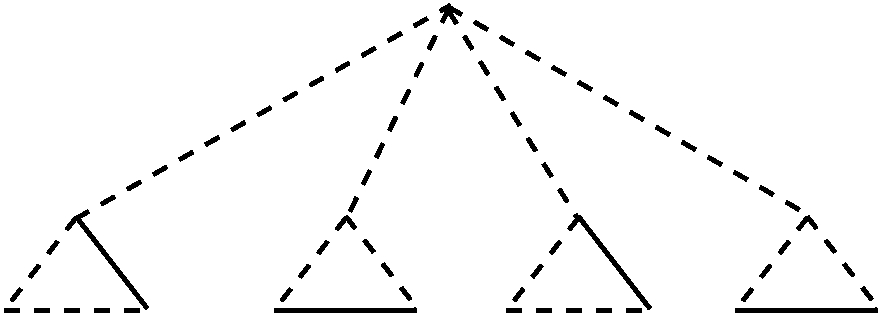
\includegraphics[width=0.5\linewidth,keepaspectratio]{opspannend5}
\end{center}
\caption{Graaf met een hybride opspannende boom\label{opspannend5}}
\end{figure}


\subsection{Minimale opspannende bomen}

Beschouwen we het volgende probleem: gegeven een aantal steden en stel
dat de kost van het bouwen van een weg tussen de steden gegeven is;
bepaal welke wegen moeten aangelegd worden om te voldoen aan (1) de
totale kost is minimaal (2) elke stad is bereikbaar vanuit elke andere
stad. Het wegennet dat daaraan voldoet moet een boom zijn, want er
kunnen geen kringen zijn (anders ware het net niet van minimale kost)
en er is een pad tussen elke twee steden. Dit soort bomen wordt
nu gedefinieerd:


 \grijs{\begin{definitie} Minimale opspannende boom\\
\textup{Voor een gewogen graaf $G$ is $T$ een \textbf{minimale opspannende
boom} indien $T$ een opspannende boom van $G$ is met het kleinste gewicht.}
\end{definitie}}

Figuur~\ref{opspannend1} laat een graaf $G$ zien, een opspannende boom $B$
en een minimale opspannende boom $T$.

\begin{figure}[ht]
\begin{center}
\includegraphics[width=0.6\linewidth,keepaspectratio]{opspannend1}
\end{center}
\caption{Een graaf met opspannende bomen\label{opspannend1}}
\end{figure}


Effici\"ente algoritmen die een minimale opspannende boom construeren
zijn gebaseerd op de volgende stelling:

 \grijs{\begin{stelling} Een boog die tot een minimale opspannende boom behoort \label{even}\\
  Gegeven een samenhangende graaf $(V,E)$, $U \subset V$ en $e$ een boog in $E$ met
  minimale lengte van alle bogen met begin in $U$ en einde in $V \backslash
  U$; er bestaat een minimale opspannende boom $T$ voor $(V,E)$ 
  zodanig dat $e \in T$.
\end{stelling}} % stelling 2.3 uit Shimon Even
\begin{proof} Neem een minimale opspannende boom $T_{0}$ voor de
graaf. Indien $e$ tot $T_{0}$ behoort is de stelling bewezen, indien
niet, voeg dan $e$ toe aan $T_{0}$. We verkrijgen $T_{1}$ die een kring
bevat (Stelling~\ref{opspannend4}) en die kring bevat $e$ alsook nog een 
boog $e' = (u,v)$
 waarbij $u \in U$ en $v \in V \backslash U$. Door uit $T_{1}$ $e'$ te
verwijderen verkrijgen we weer een opspannende boom $T$ (waarom is $T$ een
boom?) en bovendien is de 
$w(T) \leq w(T_{0})$ vermits $w(e)
\leq w(e')$. Bijgevolg is $T$ een minimale opspannende boom die $e$
bevat.
\end{proof}



\begin{algo} Prim \label{prim}\\
  Gegeven een samenhangende gewogen graaf $G(V,E)$ met een verzameling
  knopen $V =
  \{v_{1},v_{2},\ldots,v_{n}\}$.  De volgende procedure is een algoritme
  dat een minimale opspannende boom $T$ construeert.
\begin{enumerate}
\item \textbf{Initialisatie}: $T := (\{v_{1}\},\emptyset)$
\item \textbf{Stop?}: Indien $T$ $(n-1)$ bogen heeft, stop.
\item \textbf{Voeg boog toe}: 
Van alle bogen die een knoop van $T$ verbinden met een knoop die niet tot $T$
behoort, kies een boog $b$ met het kleinste gewicht en voeg
die toe aan $T$: er bestaat minstens \'{e}\'{e}n zulke boog omdat $G$
samenhangend is en $T$ nog niet alle knopen bevat; $T$ zal na
toevoeging van $b$ nog steeds kringloos zijn.
Ga naar \textbf{Stop?}.
\end{enumerate}
\end{algo}
\begin{proof} Vermits bij het einde van het algoritme $T$ een boom
is met $n$ knopen en $(n-1)$ bogen en $T$ kringloos is, is $T$ een opspannende
boom voor $G$. We moeten dus terminatie van het algoritme en
minimaliteit van $T$ bewijzen.

Een illustratie van de redenering hieronder, vind je in figuur
\ref{prim2}.

Eindigheid is eenvoudig want \textbf{Voeg boog toe} wordt slechts
$(n-1)$ keer uitgevoerd, waarna het algoritme stopt. Misschien wil je je
er nog van overtuigen dat \textbf{Voeg boog toe} altijd kan, t.t.z.
dat er altijd een boog bestaat die geen kringen introduceert in $T$.

Na \textbf{Initialisatie} bestaat $T$ uit \'{e}\'{e}n knoop en dus is $T$
een deel van een minimale opspannende boom (mob). We bewijzen nu dat
die eigenschap behouden blijft door \textbf{Voeg boog toe}: noteer met
W de knopen van $T$ en onderstel dat $T \subset T'$ met $T'$ een mob.
Noteer met $B = \{(x,y)\;|\; x \in W,\; y \in V \backslash W,\; (x,y) \in
E\}$.  Neem de kortste boog $(i,j)$ in $B$ die geen kring veroorzaakt
indien toegevoegd aan $T$. Indien $(i,j) \in T'$ dan is duidelijk dat $T
\cup \{(i,j)\} \subseteq T' = $mob. Indien $(i,j) \notin T'$ dan zal
$T' \cup \{(i,j)\}$ een kring bevatten, waarvan $(i,j)$ deel uitmaakt.
In die kring zit nog een boog $(x,y) \in B$ en door die uit $T' \cup
\{(i,j)\}$ te verwijderen krijgen we een nieuwe opspannende boom $T''$
(want bevat alle knopen en is samenhangend). De vraag is dan: is $T''$
ook minimaal? Vermits $w(i,j) \leq w(x,y)$ (zo was $(i,j)$ immers
gekozen), is $w(T'') \leq w(T')$ en bijgevolg is $T''$ een mob.
Bijgevolg is $T \cup \{(i,j)\}$ deel van een mob.

Bijgevolg is de opspannende boom door Prim geconstrueerd, een minimale
opspannende boom.
\end{proof}

\begin{figure}[ht]
\begin{center}
\includegraphics[width=0.4\linewidth,keepaspectratio]{prim2}
\end{center}
\caption{Illustratie bij Algoritme~\ref{prim} \label{prim2}}
\end{figure}


Het algoritme van Prim is een klassiek voorbeeld van een ``gulzig''
(Engels: greedy) algoritme: op elk ogenblik dat een keuze gemaakt moet
worden, wordt een keuze gemaakt die er op dat moment het beste uit
ziet, t.t.z.\ zonder te kijken naar de vorige keuzes (niet helemaal
correct) of naar de toekomstige keuzes. Niet elk gulzig algoritme
bereikt dan ook een optimaal resultaat; bv. een kortste-pad algoritme
dat op elk ogenblik een bestaand pad zou uitbreiden met de kortste
boog, geeft niet altijd een kortste pad en een gulzig schaakspeler
wint ook niet altijd. Doch in het geval van Prim werkt het perfect.

Het algoritme van Prim wordt ge\"{\i}llustreerd in Figuur~\ref{prim1}: de
initi\"ele knoop is A; de volgorde waarin de bogen worden toegevoegd,
staat bij de bogen als a,b,c \ldots h.

\begin{figure}[ht]
\begin{center}
\includegraphics[width=0.3\linewidth,keepaspectratio]{prim1} % ,height=5cm}
\end{center}
\caption{De uitvoering van Algoritme~\ref{prim} \label{prim1}}
\end{figure}


Het algoritme van Prim bouwt een mob incrementeel, t.t.z. op elk
ogenblik in het algoritme is T een mob van een deelgraaf van G. Er is
een variante op het algoritme van Prim dat deze eigenschap niet heeft:

\newpage
\begin{algo} Kruskal \label{kruskal}\\
  Gegeven een samenhangende gewogen graaf G(V,E) met een verzameling
  knopen $V =
  \{v_{1},v_{2},\ldots,v_{n}\}$.  De volgende procedure is een algoritme
  dat een minimale opspannende boom $T$ construeert.
\begin{enumerate}
\item \textbf{Initialisatie}: $T := \emptyset$
\item \textbf{Stop?}: Indien $T$ $(n-1)$ bogen heeft, stop.
\item \textbf{Voeg boog toe}: Voeg aan $T$ toe een boog $b$ met minimaal
  gewicht en die bovendien geen kring veroorzaakt indien toegevoegd
  aan $T$. 
  Ga naar {\bf Stop?}.
\end{enumerate}
\end{algo}
\begin{proof}
Eindigheid van Kruskal is analoog aan die van Prim.
Dat $T$ op het einde een opspannende boom is, is ook analoog na te gaan.
We tonen nog de minimaliteit van $T$ aan.
%
Onderstel dat $T$ geen mob is.
Noem de bogen van $T$ $b_{1},b_{2},\ldots ,b_{n-1}$ in orde van toevoeging
door het algoritme.
Laat $S$ een mob (van $G$) zijn zodanig dat $\{b_{1}, b_{2}, \ldots ,
b_{i}\} \subseteq S$ en met maximale $i$ (zulk een S bestaat en door
Stelling~\ref{even} is $i \geq 1$!) Er zijn twee mogelijkheden:
\begin{itemize}
\item
\textbf{$i = n-1$}: nu is $T = S$ en $T$ is een mob.
\item
\textbf{$i < n-1$}: dus $b_{i+1} \notin S$; laat $H$ de graaf zijn
gevormd door de bogen $\{b_{1}, b_{2}, \ldots , b_{i}\}$ en hun
knopen. Beschouw de graaf $S \cup \{b_{i+1}\} = S'$. $S'$ heeft een
kring (want een boog te veel) waarin minstens \'{e}\'{e}n boog $b$ zit
die niet tot $T$ behoort (omdat $T$ zelf kringvrij is). Dus $b \in
S$. Nu bevat $H \cup \{b\}$ geen kring, want $H \cup \{b\} \subseteq
S$ en vermits Kruskal in de $(i+1)$-de \textbf{Voeg boog toe} de boog
$b_{i+1}$ koos (om toe te voegen aan $H$), moet $w(b_{i+1}) \leq
w(b)$. Bijgevolg is $S' \backslash \{b\} = S''$ een mob. Maar nu is $S''$
een mob die $\{b_{1}, b_{2}, \ldots , b_{i+1}\}$ omvat wat in
tegenspraak is met de maximaliteit van $S$. Dus het is niet mogelijk
dat $i < n-1$.
\end{itemize}
\end{proof}

Merk op dat $T$ tijdens Kruskal's algoritme geen boom hoeft te zijn: de
uitvoering van Kruskal wordt in Figuure~\ref{kruskal1}
ge\"{\i}llustreerd op dezelfde graaf als in Figuur~\ref{prim1}.

\begin{figure}[ht]
\begin{center}
\includegraphics[width=0.3\linewidth,keepaspectratio]{kruskal1} % ,height=5cm}
\end{center}
\caption{De uitvoering van Algoritme~\ref{kruskal} \label{kruskal1}}
\end{figure}


\newpage
\section{Netwerkmodellen}

Een netwerk van verbindingen, elk met hun eigen capaciteit, kan
gemodelleerd worden als een gerichte, gewogen graaf. Als voorbeeld kan
je denken aan een wegennetwerk, een elektrisch netwerk of aan een stel
oliepijplijnen. Het belangrijkste probleem i.v.m. dit soort netwerken
is het optimaliseren van een stroming, zonder capaciteitsoverschreiding
natuurlijk. We zullen dit optimalisatieprobleem oplossen in de context
van grafentheorie. Ook andere problemen die op het eerste zicht niets
met optimalisatie van stroming te maken hebben, kunnen gemodelleerd
worden als een netwerkprobleem: personeelstoewijzing, toekenning van
resources en ook het partner-keuzeprobleem (``The marriage
problem''). 

\subsection{Transportnetwerk}

 \grijs{\begin{definitie} Transportnetwerk\\
{\rm Een \textbf{transportnetwerk} (of simpelweg een
\textbf{netwerk}) is een enkelvoudige, gewogen, gerichte graaf G die voldoet
aan
\begin{verse}
1. er is juist \'{e}\'{e}n knoop in G zonder binnenkomende bogen; deze
knoop wordt de \textbf{bron} genoemd

2. er is juist \'{e}\'{e}n knoop in G zonder buitengaande bogen; deze
knoop wordt de \textbf{put} genoemd (Engels: sink)

3.
het gewicht $C_{i,j}$ van de (gerichte) boog $(i,j)$ is postief en
wordt de \textbf{capaciteit} van de boog genoemd

4.
als de richting van de bogen vergeten wordt, dan is G samenhangend
\end{verse}
}
\end{definitie}}

Figuur~\ref{transport1} toont een netwerk: de bron is de knoop $a$ en de
put is de knoop $z$; de capaciteit van elke boog is bij de boog
geschreven. Het netwerk modelleert bijvoorbeeld een stel
eenrichtingsstraten in een stad tussen het station (knoop $a$) en de
markt (knoop $z$); de capaciteit is het aantal voertuigen dat per minuut
kan passeren door elke straat.

\begin{figure}[ht]
\begin{center}
\includegraphics[width=0.3\linewidth,keepaspectratio]{transport1} % ,height=3cm}
\end{center}
\caption{Een transportnetwerk \label{transport1}}
\end{figure}

De beperking dat een netwerk enkelvoudig moet zijn, is niet erg groot:
zowel lussen als parallelle bogen kan je wegwerken door knopen bij te
zetten op elke lus of parallelle boog; er verandert niets essentieels
aan het netwerk wat betreft de problemen die we bestuderen in deze
sectie.

 \grijs{\begin{definitie}Stroming in een netwerk \label{stroming1}
\label{stromingdef}\\
{\rm Voor een netwerk $G(V,E)$ met capaciteit $C_{i,j},\;\; i,j \in
    V$\footnotemark
    is $F$ een \textbf{stroming} als $F$ een afbeelding is
    van $E$ naar $\R^{+}$ zodanig dat\\
\begin{minipage}{12cm}
\begin{enumerate}
\item
\label{stromingdef1}
$F(i,j) \leq C_{i,j}$
\item \label{conserve1} voor elke knoop $j$ die niet de bron of de put is geldt:
\[\displaystyle \sum_{i \in V} F(i,j) = \sum_{i \in V} F(j,i)\]
\end{enumerate}
\end{minipage}\\[2mm]
We noemen $F(i,j)$ de stroming in boog $(i,j)$. Voor een knoop $j$ noemen we
$\sum_{i \in V} F(i,j)$ de stroming \textbf{naar} of \textbf{in} $j$ en
$\sum_{i \in V} F(j,i)$ de stroming \textbf{uit} $j$.
}
\end{definitie}}
\footnotetext{als er geen 
boog $(i,j)$ bestaat, dan nemen we aan dat $C_{i,j} = 0$} 

Formule~\ref{conserve1} in Definitie~\ref{stroming1} drukt het behoud
van stroming uit: alles wat binnenkomt in een knoop, gaat er weer buiten
en alles wat buitengaat, is binnengekomen; dat verhindert dat er een
ophoping of productie gebeurt in de knopen.

Figuur~\ref{stroom2} toont een stroming voor het netwerk van figuur
\ref{transport1}; de stroming is gedefinieerd door:
\begin{center}
$
\begin{array}{l}
F(a,b) = 2\\
F(b,c) = 2\\
F(c,z) = 3\\
F(a,d) = 3\\
F(d,c) = 1\\
F(d,e) = 2\\
F(e,z) = 2\\
\end{array}
$
\end{center}
en telkens naast de capaciteit van de overeenkomstige boog gezet.
\begin{figure}[ht]
\begin{center}
\includegraphics[width=0.3\linewidth,keepaspectratio]{stroom2} % ,height=3cm}
\end{center}
\caption{Een stroming in een transportnetwerk \label{stroom2}}
\end{figure}

Je kan nagaan dat Formule~\ref{conserve1} in Definitie~\ref{stroming1}
voldaan is voor elke knoop behalve de bron en de put.

Je kan ook nagaan dat de stroming uit de bron gelijk is aan de stroming in
de put:
\begin{center}
\mbox{$F(a,b)+F(a,d) = F(c,z) + F(e,z)$}.
\end{center}
Deze gelijkheid wordt veralgemeend in:

 \grijs{\begin{stelling} Bron-uit = put-in \label{bron=put}\\
Van een stroming $F$ in een netwerk $G(V,E)$ is de stroming uit de bron gelijk
aan de stroming in de put, of meer formeel: 
\[\sum_{i \in V} F(a,i) =
\sum_{i \in V} F(i,z).\]
\end{stelling}}
\begin{proof}

Het is duidelijk dat

$~~~~~~~~~~\sum_{j \in V} (\sum_{i \in V} F(i,j))  = 
                \sum_{i \in V} (\sum_{j \in V} F(i,j))
         =  \sum_{j \in V} (\sum_{i \in V} F(j,i))$


De omwisseling van de $\sum$'s mag omdat we met eindige grafen te
doen hebben. De tweede gelijkheid geldt wegens hernoeming van $i$ en $j$.

Daaruit volgt:

\begin{tabular}{c c c l}
~~~~~~~~~ &
0 & = & $\sum_{j \in V} \left(\sum_{i \in V} F(i,j) - \sum_{i \in V} F(j,i) \right)$\\
 & & & \\
 &  & = & $\left( \sum_{i \in V} F(i,z) -  \sum_{i \in V} F(z,i)\right) +
                \left(\sum_{i \in V} F(i,a) -  \sum_{i \in V} F(a,i)\right)$
    \\
 & & & \\
 &  &  & \hspace*{2cm}
       $+ \sum_{j \in V \backslash \{a,z\}} \left( \sum_{i \in V} F(i,j) -
                \sum_{i \in V} F(j,i)\right)$\\
 & & & \\
 & & = & $\sum_{i \in V} F(i,z) - \sum_{i \in V} F(a,i)$
\end{tabular}



vermits $F(z,i) = 0 = F(i,a)$ voor $\forall i \in V$ (door Definitie~\ref{stromingdef})

en $\sum_{i \in V} F(i,j) = \sum_{i \in V} F(j,i)$ voor $\forall j \in (V \backslash \{a,z\})$ (door Formule~\ref{conserve1} in Definitie~\ref{stromingdef})
\end{proof}



Op basis van Stelling~\ref{bron=put}, kunnen we nu defini\"eren:

 \grijs{\begin{definitie} Grootte van een stroming\\
\textup{De \textbf{grootte van een stroming $F$} in een netwerk $G(V,E)$
met bron $a$ en put $z$ is gedefinieerd door $\sum_{i \in V} F(a,i)$ of
$\sum_{i \in V} F(i,z)$ }
\end{definitie}}

De grootte van de stroming in Figuur~\ref{stroom2} is 5.



Het netwerkprobleem kan nu als volgt geformuleerd worden: voor een
gegeven netwerk $G$, vind de maximale stroming, of m.a.w. vind de stroming
met de maximale grootte.



Tot slot van deze sectie, nog iets over netwerken met meer dan
\'{e}\'{e}n bron of put: het netwerk in Figuur~\ref{transport2} stelt
de waterbevoorrading van de steden $A$ en $B$ voor, vanuit de bronnen $X,Y$
en $Z$ en over verdeelstations $b,c$ en $d$.

\begin{figure}[ht]
\begin{center}
\includegraphics[width=0.22\linewidth,keepaspectratio]{transport2} % ,height=3cm}
\end{center}
\caption{Een transportnetwerk met meerdere bronnen en putten \label{transport2}}
\end{figure}

Door een superbron $a$ en een superput $z$ toe te voegen aan dit netwerk,
verkrijgen we terug een gewoon netwerk: vanuit $a$ voeg je ook een
gerichte boog toe naar elke bron van het originele netwerk, en vanuit
elke oude put een gerichte boog naar $z$; de toegevoegde bogen krijgen
alle de capaciteit $\infty$.

\begin{figure}[ht]
\begin{center}
\includegraphics[width=0.507\linewidth,keepaspectratio]{transport3} % ,height=3cm}
\end{center}
\caption{Een transportnetwerk met een superbron en superput \label{transport3}}
\end{figure}

In dit nieuwe netwerk geeft een maximale stroming ook een maximale
stroming voor het oorspronkelijke netwerk.

Denk niet dat een maximale stroming uniek is: Figuur~\ref{stroom3} toont
een netwerk met oneindig veel maximale stromen, nl. voor alle i,j die
voldoen aan $i+j = 5$ en $0 \leq i,j \leq 3$.

\begin{figure}[ht]
\begin{center}
\includegraphics[width=0.3\linewidth,keepaspectratio]{stroom3} % ,height=2.5cm}
\end{center}
\caption{Een netwerk met oneindig veel maximale stromen\label{stroom3}}
\end{figure}


\subsection{Maximale stroming}

We zullen een algoritme zien om een maximale stroming te berekenen; 
het basisidee is eenvoudig: vertrek van een stroming en verbeter die totdat
dat niet meer mogelijk is; je hebt nu een maximale stroming. Een
intu\"{\i}tieve beschrijving van hoe je een stroming verbetert, gaat als
volgt:
\begin{itemize}
\item
neem een pad $P$ van de bron $a$ naar de put $z$
\item
zoek het minimum $\Delta$ van $C_{b} - F(b)$ over alle bogen $b \in P$
\item
bepaal de nieuwe stroming langs het pad $P$ door bij elke $F(b)$ $\Delta$ 
bij te tellen
\end{itemize}

Een paar opmerkingen bij dit voorschrift:
\begin{itemize}
\item de operatie verhoogt de stroming enkel als het pad $P$ (toevallig)
  zo is dat $\Delta > 0$
\item de beschrijving geldt alleen voor een pad waarvan elke boog de
goede richting heeft, maar
\item we mogen niet alleen paden van $a$ naar $z$ zoeken langs de
gerichte bogen: bekijk Figuur~\ref{transport4}; daarin zie je dat geen
enkel pad van $a$ naar $z$ met enkel goede bogen ``verbeterd'' kan
worden met bovenstaande methode; maar de stroming langs het pad
$(a,b,c,z)$ kan wel verbeterd worden door de stroming getoond in
Figuur~\ref{transport5};

\begin{figure}[ht]
\begin{center}
\subfigure[Een niet maximale stroming]{\includegraphics[width=0.3\linewidth,keepaspectratio]{transport4} \label{transport4}}\hspace{1.2cm}
\subfigure[Een verbeterde stroming langs een pad met omgekeerde boog]{\includegraphics[width=0.3\linewidth,keepaspectratio]{transport5} \label{transport5}}
\end{center}
\caption{Verbetering van stroming}
\end{figure}

we moeten dus ook paden beschouwen waarvan bogen ``omgekeerd'' lopen
en we moeten voor die verkeerde bogen niet iets optellen bij de
stroming, maar er iets aftrekken: als een ``omgekeerde'' boog een stroming
draagt kan het immers zijn dat er alleen maar iets rondstroomt zonder
ooit de put te bereiken; we formaliseren dat als volgt:
\end{itemize}

 \grijs{\begin{definitie} Goede en slechte boog\\
\textup{In een gerichte graaf $G(V,E)$ met pad $(v_{1},v_{2},\ldots ,v_{n})$
noemen we de boog $(v_{i},v_{i+1})$ \textbf{goed} (gericht) indien
$(v_{i},v_{i+1}) \in E$ en anders \textbf{slecht} (gericht)}
\end{definitie}}

In een pad $P$ zullen we de goede bogen noteren door $P_{+}$ en de
slechte door $P_{-}$.


 \grijs{\begin{stelling} Verbeteren van een stroming
\label{verbeterstroming}\\
Laat $P$ een pad zijn van $a$ naar $z$ in een netwerk $G(V,E)$, waarbij
\begin{verse}
1.
$\forall (i,j) \in P_{+}$: $F(i,j) < C_{i,j}$

2. 
$\forall (i,j) \in P_{-}$: $0 < F(i,j)$
\end{verse}

Laat bovendien $\Delta = min(min_{(i,j) \in P_{+}}
\{C_{i,j}-F(i,j)\},min_{(i,j) \in P_{-}} \{F(i,j)\})$; definieer de
functie $F'$ als volgt:

\begin{eqnarray*}
F'(i,j) & = & F(i,j) \quad \forall (i,j) \notin P\\
        & = & F(i,j) + \Delta \quad \forall (i,j) \in P_{+}\\
        & = & F(i,j) - \Delta \quad \forall (i,j) \in P_{-}
\end{eqnarray*}

Dan is $F'$ een stroming waarvan de grootte $\Delta$ meer is dan die van $F$.

\end{stelling}}
\begin{proof} Om na te gaan dat $F'$ een stroming is, moeten we
\ref{stromingdef1} en~\ref{conserve1} van Definitie~\ref{stromingdef}
bewijzen: beide zijn niet moeilijk.

Dat de stroming met $\Delta$ verbeterd is, volgt uit het feit dat de
stroming van de boog $(a,\_) \in P$ (en die is goed - waarom?) met
$\Delta$ is verhoogd en de stroming door de andere bogen die vertrekken
in $a$ niet is veranderd.  \end{proof}



E\'{e}n van de gevolgen van de stelling over de verbetering van de
stroming, is dat bij een maximale stroming $F$ elk pad van $a$ naar $z$,
minstens \'{e}\'{e}n goede boog heeft met $C_{i,j} = F(i,j)$ of
\'{e}\'{e}n slechte boog met $F(i,j) = 0$; zoniet kon de stroming
verbeterd worden langs dat pad.

We zouden ook graag de volgende eigenschappen hebben:
\begin{itemize}
\item
als een stroming geen enkel pad van $a$ naar $z$ heeft dat kan verbeterd
worden (volgens de methode van Stelling~\ref{verbeterstroming}) dan is
de stroming maximaal - dit lijkt voor de hand liggend, maar is niet
triviaal te bewijzen!
\item
een algoritme om de flow te maximaliseren bestaat erin om
een pad te zoeken dat aan de voorwaarden van stelling
\ref{verbeterstroming} voldoet, de stroming langs het pad te verbeteren en
dat te herhalen tot er geen zulk pad meer is - indien voorgaand
puntje waar is en de procedure eindigt, dan levert dit inderdaad een
maximale stroming op.
\end{itemize}

We zullen beide eigenschappen formeel aantonen. We beschrijven eerst
een klassiek algoritme dat een voorbeeld is van een ``labeling
procedure''. Je hebt vroeger al een algoritme gezien dat labels
gebruikte nl. het kortste-pad algoritme van Edgser Dijkstra: knopen kregen
daarbij een label met informatie. In het volgende algoritme gebruiken
we een dubbel label: informeel is de eerste component van
het label de knoop waarvan je kwam (en daarom zal de startknoop een
lege eerste component in zijn label hebben) en de tweede component van
het label zal de $\Delta$ uit Stelling~\ref{verbeterstroming} zijn van
het pad dat tot dan is gevonden.

\begin{algo} Constructie van een maximale stroming.
\label{maxflow}\\
Laat $G(V,E)$ een netwerk zijn met bron $a$ en put $z$ en capaciteit $C$,
waarbij alle capaciteiten positief en geheel zijn. Onderstel een
orde op de knopen met $a = v_{0}, v_{1}, \ldots , v_{n} = z$.

Met ${\cal B}$ zullen we de verzameling beschouwde knopen aanduiden;
met ${\cal L}$ de verzameling van knopen met een label; de operaties
op ${\cal B}$ zullen we expliciet maken; die op ${\cal L}$ zijn impliciet.

\begin{enumerate} \item \textbf{Initialisatie}:
Definieer $\forall (i,j) \in E: F(i,j) = 0$

\item
\textbf{Label de bron}: Geef $a$ het label $(\_,\infty)$;  zet ${\cal B} = \emptyset$

\item
\textbf{Aangekomen?}: Indien $z$ een label heeft, verbeter de stroming
en ga terug naar \textbf{Label de bron}.

Verbeter de stroming gaat als volgt: er is juist \'{e}\'{e}n pad $P$ van $a$ naar
$z$ dat achteruit kan geconstrueerd worden te vertrekken van $z$, dan
de eerste component van het label van $z$ en zo verder tot in $a$. De
tweede component van het label van $z$ is een grootheid $\Delta$ die
nu wordt bijgeteld bij $F$ voor goede bogen in $P$ en afgetrokken van
$F$ voor slechte bogen van $P$. Daarna worden alle labels in heel het
netwerk gewist.

\item
\textbf{Kies volgende knoop}: Indien ${\cal L} \setminus {\cal B} =
\emptyset$, \textbf{stop}: de stroming $F$ is maximaal.

Noem $v$ de nog niet beschouwde knoop $v_{i}$ met een label en met
kleinste index $i$.
\item
\textbf{Label buren}: Stel dat het label van $v$ gelijk is aan
$(\alpha,\Delta)$. Behandel nu elke boog van de vorm $(v,w)$ of
$(w,v)$ in de volgorde $(v,v_{0})$, $(v_{0},v)$, $(v,v_{1})$, $(v_{1},v)$,
$\ldots $ waarbij $w$ nog geen label heeft.
\begin{itemize}
\item
voor elke boog $(v,w)$ (dus een boog die wegloopt uit $v$):
indien $F(v,w) < C_{v,w}$ geef $w$ het label $(v,min\{\Delta,C_{v,w}-F(v,w)\})$
anders geef je $w$ geen label
\item
voor elke boog $(w,v)$ (dus een boog die toekomt in $v$):
indien $F(w,v) > 0$ geef $w$ het label $(v,min\{\Delta,F(w,v)\})$
anders geef je $w$ geen label
\end{itemize}
Ga naar \textbf{Aangekomen?}
\end{enumerate}
\end{algo}
\begin{proof}
~\\
\begin{itemize}
\item
\textbf{Eindigheid}:
Punt 3 in het algoritme is cruciaal: zolang de uitgang \textbf{stop}
niet genomen wordt, wordt punt 3 herhaaldelijk uitgevoerd. Vanuit punt
3, gaat de uitvoering ofwel naar punt 2 of punt 4. De overgang van
punt 3 naar punt 2 kan maar een eindig aantal keer gebeuren, want die
overgang impliceert dat de stroming verbeterd wordt met $\Delta > 0$;
$\Delta$ is geheel omdat alle capaciteiten geheel zijn en vermits de
maximale stroming begrensd is (door de som van de capaciteiten van de
bogen die vertrekken in de bron) kan de gegeven stroming dus slechts
een eindig aantal keer verbeterd worden. Na een eindig aantal
overgangen van punt 3 naar punt 2, wordt dus steeds opnieuw de
overgang van punt 3 naar punt 4 genomen. In punt 4 wordt telkens een
knoop toegevoegd aan ${\cal B}$ (die nooit meer terug op $\emptyset$
wordt gezet). Bijgevolg zal na verloop van tijd ${\cal L}={\cal B}$ en
op dat moment stopt het algoritme.
\item
\textbf{Maximaliteit}: we stellen het bewijs nog even uit tot we
Stelling~\ref{maxflowmincut} hebben gezien.
\end{itemize}
\end{proof}

Merk op dat het Algoritme~\ref{maxflow} niet alle maximale stromen
vindt: zie Figuur~\ref{stroom3}.


 \grijs{\begin{definitie} Snede van een netwerk\\
  \textup{Een \textbf{snede} van een netwerk $G(V,E)$ met bron $a$ en put
    $z$, is een 2-tal $(P,\overline{P})$ 
    zodanig dat $a \in P$, $z \in \overline{P}$, $P
    \cup \overline{P} = V$ en $P \cap \overline{P} = \emptyset$ }
\end{definitie}}

We kunnen een snede tekenen door een lijn die de knopen van het
netwerk in twee verzamelingen verdeelt: op Figuur~\ref{snede1} is een
snede aangegeven met een stippellijn.

\begin{figure}[ht]
\begin{center}
\includegraphics[width=0.3\linewidth,keepaspectratio]{snede1} % ,height=4cm}
\end{center}
\caption{Een netwerk met een stroming en een snede\label{snede1}}
\end{figure}

We kunnen nagaan hoeveel stroming er globaal loopt over de snede,
t.t.z. van links naar rechts in de tekening van een netwerk: daarbij
moeten we een boog van P naar $\overline{P}$ positief rekenen en een
omgekeerde boog negatief; voor het net in Figuur~\ref{snede1} wordt
dat: \mbox{$~~~~~~~~F(c,e) + F(b,d) - F(d,c) = 2+1-1=2$ }

Vergelijken we die grootheid met de stroming (in {\em a} of {\em z}) dan zien we
dat die ook gelijk is aan 2! Is dit toeval of niet? We kunnen ook
proberen een afschatting te maken van hoeveel stroming er maximaal van
links naar rechts over de snede kan lopen, door optimistisch te
veronderstellen dat er misschien een stroming bestaat die voor alle
goede bogen over de snede maximaal is, t.t.z. gelijk aan de capaciteit
van die boog en voor alle slechte bogen nul. We zullen die grootheid
de capaciteit van de snede noemen. Voor hetzelfde voorbeeld geeft dat: 
\mbox{$~~~~~~~~C_{c,e} + C_{b,d} = 2+3=5$}

En het lijkt alsof capaciteit van de snede groter is dan de stroming
van de snede en ook groter dan de maximale stroming (je kan nagaan dat
die 4 is). Is dit toeval? We bekijken deze vragen in een meer
formeel kader:

 \grijs{\begin{definitie} Capaciteit $C(P,\overline{P})$ van een snede\\
  \textup{De \textbf{capaciteit van een snede} $(P,\overline{P})$ is
    $C(P,\overline{P}) = \displaystyle
    \sum_{i \in P} \sum_{j \in \overline{P}} C_{i,j}$}
\end{definitie}}

 \grijs{\begin{stelling} \label{snedestroming}
De capaciteit van een snede is niet kleiner dan een stroming, m.a.w.
\[\sum_{i \in P} \sum_{j \in \overline{P}} C_{i,j} \geq \sum_{i \in V} F(a,i).\]
\end{stelling}}
\begin{proof}
\begin{eqnarray*}
\sum_{i \in V} F(a,i) & = & 
                \sum_{i \in V}(F(a,i) - F(i,a)) +
                \sum_{j \in P \backslash \{a\}} \sum_{i \in V}(F(j,i) - F(i,j))\\
        & = & \sum_{j \in P} \sum_{i \in V} (F(j,i) - F(i,j)) \\
        & = & \sum_{j \in P} \sum_{i \in P} F(j,i) +
                \sum_{j \in P} \sum_{i \in \overline{P}} F(j,i) -
                \sum_{j \in P} \sum_{i \in P} F(i,j) -
                \sum_{j \in P} \sum_{i \in \overline{P}} F(i,j)\\
        & = & \sum_{j \in P} \sum_{i \in \overline{P}} F(j,i) -
                \sum_{j \in P} \sum_{i \in \overline{P}} F(i,j)\\
        & \leq & \sum_{j \in P} \sum_{i \in \overline{P}} F(j,i)\\
        & \leq & C(P,\overline{P})
\end{eqnarray*}
\end{proof}

Merk op dat de derde laatste regel van de stelling inderdaad aantoont
dat de stroming gelijk is aan de stroming die door de snede loopt.



Een \textbf{minimale} snede is een snede met minimale capaciteit.
Vorige stelling impliceert direct dat de maximale stroming kleiner of
gelijk is aan de capaciteit van de minimale snede. Het verband tussen
beide grootheden is nog sterker:


 \grijs{\begin{stelling} Max flow - min cut \label{maxflowmincut}\\
  Voor een snede $(P,\overline{P})$ en stroming $F$ in een net $G(V,E)$ 
  geldt dat als 
\[C(P,\overline{P})=F\mbox{ \ \ (of dus als }
\sum_{i \in P} \sum_{j \in \overline{P}} C_{i,j} = \sum_{i \in V} F(a,i)
 \mbox{ )}\]
 dan is de stroming maximaal en de snede minimaal.\\
  Bovendien is die gelijkheid equivalent met
\begin{enumerate}
\item
$\forall i \in P, j \in \overline{P}: F(i,j) = C_{i,j}$ en
\item
$\forall i \in \overline{P}, j \in P: F(i,j) = 0$
\end{enumerate}
t.t.z. goede bogen over de snede hebben een stroming gelijk aan hun
capaciteit en slechte bogen een nul stroming.
\end{stelling}}
\begin{proof}
Volgt onmiddellijk uit de ongelijkheden van Stelling~\ref{snedestroming}
\end{proof}



Merk op dat we niet bewezen dat er voor elke maximale stroom een
minimale snede is met die gelijkheid
noch omgekeerd.



Figuur~\ref{snede2} toont een maximale stroom met minimale snede.

\begin{figure}[ht]
\begin{center}
\includegraphics[width=0.35\linewidth,keepaspectratio]{snede2} % ,height=4cm}
\end{center}
\caption{Een netwerk met een maximale stroming en een minimale snede\label{snede2}}
\end{figure}




Nu kunnen we bewijzen dat Algoritme~\ref{maxflow} inderdaad eindigt
met een maximale stroming.



\begin{proof} (van Stelling~\ref{maxflow})\\
Op het ogenblik dat het algoritme stopt, is er een verzameling $P$ van
knopen met een label ($a \in P$) en $\overline{P}$ van knopen zonder label 
($z \in \overline{P}$). $(P,\overline{P})$ vormt dus een snede. 
Beschouw een boog die
vertrekt in $i$, t.t.z. een boog $(i,j)$ met $i \in P$ en $j \in \overline{P}$.
Vermits i een label heeft moet $F(i,j) = C_{i,j}$ anders zou $j$ een
label hebben gekregen. Beschouw nu een aankomende boog in $i$, t.t.z.
een boog $(j,i)$ met $i \in P$ en $j \in \overline{P}$. Vermits $i$ een label
heeft moet $F(j,i) = 0$ anders zou $j$ een label hebben gekregen. Samen
met Stelling~\ref{maxflowmincut} verkrijgen we dat $F$ maximaal is.
\end{proof}



We zien dus dat het algoritme tegelijkertijd een maximale stroming
construeert en een minimale snede. We tonen de opeenvolgende stappen
in Algoritme~\ref{maxflow} in de reeks Figuren~\ref{maxflow1} en~\ref{maxflow2}:

\begin{figure}[ht]
\begin{center}
\subfigure[Na initialisatie en labeling bron a]{\includegraphics[width=0.4\linewidth,keepaspectratio]{maxflow1} \label{maxflow1}} \hspace{1cm}
\subfigure[Na een labeling die $z$ bereikt]{\includegraphics[width=0.4\linewidth,keepaspectratio]{maxflow2} \label{maxflow2}}
\end{center}
\caption{Illustratie 1 bij Algoritme~\ref{maxflow}}
\end{figure}

Als orde op de knopen kozen we $(a,c,d,b,z)$. Vanuit $a$ krijgt dus eerst
$d$ en dan $b$ een label. Vanuit $d$ wordt dan $c$ gelabeld; vanuit $d$ wordt 
$b$ niet gelabeld omdat $b$ al een label heeft. Vervolgens  krijgt $z$
een label vanuit $c$: er is nu een pad vanuit $a$ naar $z$, te zien in
Figuur~\ref{maxflow2}. De stroming wordt aangepast: het resultaat is
te zien in Figuur~\ref{maxflow3}.

\begin{figure}[ht]
\begin{center}
\subfigure[De stroming is een eerste maal verbeterd]{\includegraphics[width=0.35\linewidth,keepaspectratio]{maxflow3} \label{maxflow3}} \hspace{1cm}
\subfigure[Een tweede labeling heeft $z$ bereikt]{\includegraphics[width=0.35\linewidth,keepaspectratio]{maxflow4} \label{maxflow4}}
\end{center}
\caption{Illustratie 2 bij Algoritme~\ref{maxflow}}
\end{figure}

De labeling herbegint in de situatie van Figuur~\ref{maxflow3}. Vanuit
$a$ krijgt $d$ nu geen label, want de stroming door de boog $(a,d)$ is al
maximaal. Vanuit $b$ krijgt $c$ geen label, want de boog $(c,b)$ is
``slecht'' en de stroming $ = 0$. Dus krijgt $d$ een label vanuit $b$, en
vermits de capaciteit van de boog $(b,d)$ (3) kleiner is dan de $\Delta$
van $b$ (7 op dat ogenblik) krijgt het label van $d$ een $\Delta =
3$. Vanuit $d$ krijgt $c$ een label en vermits de overschotcapaciteit van
de boog $(d,c)$ nog 2 is, krijgt $c$ een $\Delta = 2$. Vanuit $c$ kan enkel
nog $z$ gelabeld worden: de eindsituatie is te zien in figuur
\ref{maxflow4}. Weerom kan de stroming langs het bekomen pad aangepast
worden, wat resulteert in Figuur~\ref{maxflow5}.

\begin{figure}[ht]
\begin{center}
\subfigure[De stroming is een tweede maal verbeterd]{\includegraphics[width=0.35\linewidth,keepaspectratio]{maxflow5} \label{maxflow5}} \hspace{1cm}
\subfigure[De labeling bereikt $z$ niet meer: de snede is minimaal, de stroming maximaal]{\includegraphics[width=0.35\linewidth,keepaspectratio]{maxflow6} \label{maxflow6}}
\end{center}
\caption{Illustratie 3 bij Algoritme~\ref{maxflow}}
\end{figure}

Op dit ogenblik is de stroming al maximaal, maar daarom stopt het
algoritme nog niet: er wordt nog eens een poging gedaan om een pad van
$a$ naar $z$ te maken, met bogen die nog overschotcapaciteit hebben. De
laatste ronde van labelen begint in de situatie van figuur
\ref{maxflow5}: vanuit $a$ kan enkel $b$ een label krijgen (de capaciteit
van boog $(a,d)$ is al opgebruikt) en boog $(b,d)$ heeft ook nog wat
overschotcapaciteit, maar dan is het gedaan: de labeling stopt bij
Figuur~\ref{maxflow6}. We hebben $P = \{a,b,d\}$ en $\overline{P} =
\{c,z\}$ en de snede is minimaal.

Voer zelf het algoritme uit op de netwerken in Figuur~\ref{maxflow7}, met
als orde op de knopen: $(a,b,c,d,e,z)$.

\begin{figure}[ht]
\begin{center}
\includegraphics[width=0.6\linewidth,keepaspectratio]{maxflow7} % ,height=3.2cm}
\end{center}
\caption{Twee netwerken om op te oefenen \label{maxflow7}}
\end{figure}

Het vinden van een maximale stroming in een netwerk, komt neer op het
zoeken van (gehele) getallen $F(i,j)$ zodanig dat
\begin{itemize}
\item
$\sum_{j} F(a,j)$ maximaal is
\item
$0 \leq F(i,j) \leq C_{i,j}$ voor gegeven $C_{i,j}$
\item
$\forall j: \sum_{i} F(i,j) = \sum_{i} F(j,i)$
\end{itemize}

Dit soort problemen wordt ook opgelost in lineaire programmatie,
m.b.v. het simplex algoritme: je leert er elders misschien meer over.

\subsection{Matching}

Beschouw het volgende probleem: er zijn 4 studenten ($A,B,C$ en $D$) en
die willen elk apart naar het monitoraat dat open is op 5 tijdstippen
$(a,b,c,d$ en $e)$. Elk van die studenten heeft zijn voorkeur voor
\'{e}\'{e}n of meer tijdstippen laten blijken en nu is het aan het
monitoraat om een afspraakagenda vast te leggen zodat elk van die
studenten kan komen op een tijdstip dat zijn voorkeur heeft. Het is
duidelijk dat dit niet altijd mogelijk is: indien bijvoorbeeld
studenten $A$ en $B$ beiden als enige voorkeur het tijdstip $a$ hebben, dan
is het al onmogelijk. Maar zelfs als het mogelijk is, is het niet
triviaal om dit probleem op te lossen, zeker niet als er veel meer dan
4 studenten en veel meer dan 5 tijdstippen zijn.

Op het eerste zicht heeft dit probleem niet veel met grafen te maken,
maar laten we toch een graaf maken van dit probleem: de knopen zijn de
studenten en de tijdstippen en er is een gerichte boog tussen een
student en een tijdstip, indien die student dat tijdstip verkiest.
Stel dat $A$ voorkeur $\{b,c\}$ heeft, $B$ heeft $\{a,b\}$, 
$C \{d,e\}$ en $D$
$\{b,c,e\}$. Dan krijgen we Figuur~\ref{matching1}

\begin{figure}[ht]
\begin{center}
\includegraphics[width=0.17\linewidth,keepaspectratio]{matching1} % ,height=4cm}
\end{center}
\caption{Graaf voor het toekenningsprobleem\label{matching1}}
\end{figure}

We hebben een tweeledige, gerichte graaf. Het verband met de vorige
sectie zien we als we een bron en put toevoegen en elke boog
capaciteit gelijk aan \'{e}\'{e}n geven. Zie Figuur~\ref{matching2}.

\begin{figure}[ht]
\begin{center}
\includegraphics[width=0.5\linewidth,keepaspectratio]{matching2} % ,height=4cm}
\end{center}
\caption{Netwerk voor het toekenningsprobleem: alle bogen hebben capaciteit = 1\label{matching2}}
\end{figure}

Als we nu een maximale 
gehele
stroming $F$ in dat netwerk vinden en de waarde
van die maximale stroming is 4 (het aantal studenten) dan hebben we
ook een toekenning van de studenten aan de tijdstippen: een boog $e$ van
een student naar een tijdstip met $F(e) = 1$ is zulk een toekenning.
Figuur~\ref{matching3} toont een maximale stroming (de stroming met
waarde \'{e}\'{e}n loopt door de bogen in stippellijn). De oplossing
geeft de toekenning $(A,b)$, $(B,a)$, $(C,d)$, $(D,e)$. We hebben een
volledige toekenning of matching.

\begin{figure}[ht]
\begin{center}
\includegraphics[width=0.5\linewidth,keepaspectratio]{matching3} % ,height=4cm}
\end{center}
\caption{Een oplossing voor het toekenningsprobleem \label{matching3}}
\end{figure}

Het is ook mogelijk dat de maximale stroom kleiner is dan het aantal
studenten (voor een andere voorkeur natuurlijk); dan geeft de maximale
stroming enkel een maximale matching.

Meer formeel nu:

 \grijs{\begin{definitie}
{\rm Voor een gerichte, tweeledige graaf $G(V \cup W,E)$ waarbij $V
\cap W = \emptyset$ en $E \subseteq V \times W$, is $M$ een
\textbf{overeenkomst} of \textbf{matching} indien
\begin{verse}
\hspace*{1ex}$\bullet$
$M \subseteq E$ en

\hspace*{1ex}$\bullet$
$\forall (x,y),\;(i,j) \in M:$ indien $(i,j) \neq (x,y)$ dan is
$i \neq x$ en $j \neq y$
(t.t.z. in elke knoop komt hoogstens \'{e}\'{e}n boog aan en er vertrekt er hoogstens \'{e}\'{e}n)
\end{verse}
Een \textbf{maximale} matching heeft een
maximaal aantal bogen in M. Een matching is \textbf{volledig} indien
$\forall v \in V,\; \exists w\in W:\; (v,w) \in M$.
}
\end{definitie}}

Een gerichte, tweeledige graaf $G(V \cup W,E)$ waaraan een bron en put
wordt toegevoegd, bogen van de bron naar de knopen in $V$ en bogen van
de knopen in $W$ naar de put, en waar aan elke boog de capaciteit
\'{e}\'{e}n wordt toegekend, noemen we het \textbf{matching netwerk}
dat van $G$ is afgeleid.



De volgende stelling formaliseert de overeenkomst tussen een maximale
stroming in een matching netwerk en een maximale matching.
Een $gehele$ stroming $F$ is zodanig dat $F$ enkel gehele waarden heeft.

 \grijs{\begin{stelling}
Voor een gerichte, tweeledige graaf $G(V \cup W,E)$ waarbij $V
\cap W = \emptyset$ en $E \subseteq V \times W$  geldt dat
\begin{verse}
\hspace*{1ex}$\bullet$
Een gehele stroming $F$ in het overeenkomstige matching netwerk, geeft een
matching in $G$: $v \in V$ komt overeen met $w \in W$ als en slechts als $F(v,w) = 1$

\hspace*{1ex}$\bullet$
Een maximale gehele stroming komt overeen met een maximale matching.

\hspace*{1ex}$\bullet$
Een gehele stroming met waarde $\#V$ komt overeen met een volledige matching.
\end{verse}
\end{stelling}}
\begin{proof}
Het bewijs van de stelling mag je zelf uitwerken.
\end{proof}



Als we ge\"{\i}nteresseerd zijn in een volledige matching, dan is er soms
een vlugge test die aantoont dat er geen volledige matching bestaat
(zodat zoeken ernaar vermeden kan worden): het is duidelijk dat als $n$
studenten samen minder dan $n$ verschillende voorkeuren hebben opgegeven, ze niet
allen hun zin kunnen krijgen. Veralgemeend betekent dat:
\begin{itemize}
\item
definieer de afbeelding\footnote{${\cal P}(S)$ stelt de
machtsverzameling van S voor}

\begin{center}
$
\begin{array}{lrcl}
R: & {\cal P}(V) & \rightarrow & {\cal P}(W)\\
   & S    & \mapsto     & 
                \{w\in W \;|\; \exists v \in S \mbox{ met }(v,w) \in E\}
\end{array}
$
\end{center}
\item
Indien G een volledige matching heeft, dan moet $\#S \leq \#R(S),\;
\forall S \subseteq V$
\end{itemize}

De Engelse wiskundige Philip Hall bewees in 1935 ook het omgekeerde:

 \grijs{\begin{stelling} De trouwstelling van Hall \label{hall}\\
Een gerichte, tweeledige graaf $G(V \cup W,E)$ waarbij $V
\cap W = \emptyset$ en $E \subseteq V \times W$, heeft een volledige
matching als en slechts als $\#S \leq \#R(S),\; \forall S \subseteq V$
\end{stelling}}
\begin{proof}
Als $G$ een volledige matching heeft, is zeker $\#S \leq \#R(S), \forall
S \subseteq V$: dat hebben we voordien al geargumenteerd. We bewijzen
nu het omgekeerde.

We stellen $m = |V|$. We bewijzen nu door inductie op $m$ dat de
voorwaarde voldoende is. In het basisgeval $m=1$ is het duidelijk dat
er een volledige matching bestaat. Stel nu $m \geq 2$. Dan zijn er
twee gevallen te onderscheiden:

\begin{enumerate}
\item 
Stel dat voor alle $S$ zodanig dat $\emptyset \neq S \subsetneq V$ het
waar is dat $|S| + 1 \leq |R(S)|$. Neem dan een willekeurige boog
$(v,w)$ met $v \in V$ en beschouw de graaf $G' = G \setminus
\{v,w\}$. $G'$ voldoet aan de voorwaarde van Hall zijn $V'$ is strict
kleiner dan $m$: door de inductiehypothese weten we dat $G'$ een
volledige matching heeft. Voeg daaraan de boog $(v,w)$ toe om een
volledige matching voor $G$ te bekomen.

\item
Stel nu dat een $S$ bestaat met $\emptyset \neq S \subsetneq V$ en $|S| =
|R(S)|$. Beschouw nu de subgrafen $G_1$ ge\"induceerd door de knopen
$S \cup R(S)$, en $G_2$ ge\"induceerd door $(V\setminus S) \cup (W \setminus
R(S)$. Toon aan dat $G_1$ en $G_2$ beide aan de voorwaarde van Hall
voldoen, en dus elk een volledige matching hebben: neem daarvan de
unie, en je hebt een volledige matching voor $G$. Figuur \ref{hallfig}
illustreert de constructie.
\end{enumerate}
\end{proof}


\begin{figure}[h]
\begin{center}
\includegraphics[height=0.4\textheight,keepaspectratio]{hall}
\caption{De stippellijnen behoren tot de oorspronkelijke graaf, maar
niet tot $G_1$ of $G_2$}\label{hallfig}
\end{center}
\end{figure}


De stelling van Hall~\ref{hall} kan toegepast worden op partnerkeuzes,
vandaar de naam.





% http://myweb.facstaff.wwu.edu/sarkara/hall.pdf geeft een mooier bewijs
% van de stelling van Hall, eentje waarvoor geen kennis van netwerken
% nodig is.

% Zoek ook eens het {\em Stable Marriage Problem} op ...

\newpage

\section{Referenties}

\begin{itemize}
\item
Richard Johnsonbaugh ``Discrete Mathematics'', MacMillan, 1984
\item
Shimon Even ``Graph Algorithms'', Pitman, 1979
\item
Ralph P. Grimaldi ``Discrete and Combinatorial Mathematics''
\item
William Barnier, Jean B. Chan ``Discrete Mathematics''
\item
Michael Townsend ``Discrete Mathematics: Applied combinatorics and \\
graph theory''
\end{itemize}


